\chapter{Introduction} \label{chap:intro}


%###############################################################################################################################
%###############################################################################################################################
%###############################################################################################################################
\section{Nuclear Fusion}%
\label{sec:intro_whatisfusion}

Nuclear fusion is a reaction which combines multiple light nuclei together into heavier nuclei.
If the products of the reaction are more tightly bound than the reactants, excess energy is also released to the products.
Broadly, the binding energy per nucleon of common nuclear isotopes increases with atomic mass up to iron, ${}^{56}\text{Fe}$, and decreases afterwards, as is shown in Fig.~\ref{fig:intro_BEperNucleon}.
The reverse process, nuclear fission, operates by splitting heavy nuclei into lighter products, thus energy is released via fusion by combining elements up to iron and via fission down to iron.
In 2023, fission made up approximately 9.1\% of the global electricity mix~\cite{emberinstitute_statistical_2024}.
Like fission, fusion energy would be carbon free at the point of production, but it would also offer further distinct advantages.
Fusion power plants would not produce energy via potentially dangerous chain reactions and would generate little-to-no long-lived nuclear waste, depending on the specific fuel that was used.
In comparison with other low-carbon power sources, including wind and solar, studies have shown that fusion energy could have a competitive \ac{LCOE}, which is a metric that compares the economic costs of a power plant over its lifetime to the value of energy produced~\cite{griffiths_commercialisation_2022}.
Performing controlled nuclear fusion on Earth for energy production has been an active area of research for many decades and many significant scientific and engineering challenges remain to be resolved, in order to make it a viable energy source.

The likelihood of two reactants undergoing a specific fusion reaction is described by the cross-section of the interaction,
\begin{equation}
    \label{eq:intro_cross_sec}
    \sigma(E) = \frac{S(E)}{E} e^{-E_G/E},
\end{equation}
which is a function of the centre of mass energy, $E$, the `astrophysical $S$-factor', $S(E)$, which is a weakly varying function of energy for many typically deployed reactants and the Gamow Energy, $E_G$~\cite{atzeni_physics_2004}.
The exponential term in Eq.~\ref{eq:intro_cross_sec} is related to the probability of reactants tunnelling through the energy barrier, due to electrostatic Coulomb repulsion.
One approach to achieving the energies required to overcome this barrier are `beam-target' configurations, wherein a high energy beam of reactants is focussed onto a stationary target, has proven unviable~\cite{rider_general_1995}.
Thermonuclear fusion is the alternative approach, wherein the bulk fuel is heated to sufficient temperatures that the particles in the high-energy tail of the distribution have sufficient energy to undergo fusion reactions.
For a fuel is in thermal equilibrium, the high particle energies required to overcome the Coulomb barrier, $\mathcal{O}(100)\ \text{keV}$, are well above ionisation energies, $13.6\ \text{eV}$ for Hydrogen, so the fuel will be in the plasma state.
If the fusion products are able to deposit a sufficient fraction of their energy back into the fuel, then a self-sustaining fusion reaction is possible, where the high temperatures required for the reactants to fuse is maintained.
For a fusion reaction with reactants labelled by 1 and 2, the number of fusion reactions per unit time and volume is known as the `volumetric reaction rate',
\begin{equation}
    \label{eq:intro_reacrate}
    R_{12} = \frac{n_1 n_2}{1+\delta_{12}} \langle \sigma v \rangle,
\end{equation}
where $v$ is the relative velocity of a pair of reactants, $\delta_{12}$ is the Kronecker delta, which accounts for double counting of species and the `averaged reactivity' $\langle \sigma v \rangle$ is defined as the integral over the velocity distribution,
\begin{equation}
    \label{eq:intro_reactivity}
    \langle \sigma v \rangle \equiv \int_0^{\infty} \sigma(E) v f(v)\ \text{d}v.
\end{equation}
Eq.~\ref{eq:intro_reacrate} explicitly demonstrates that achieving a high fuel density, can significantly enhance reaction rates due to the square dependence.

\begin{figure}[t!]
    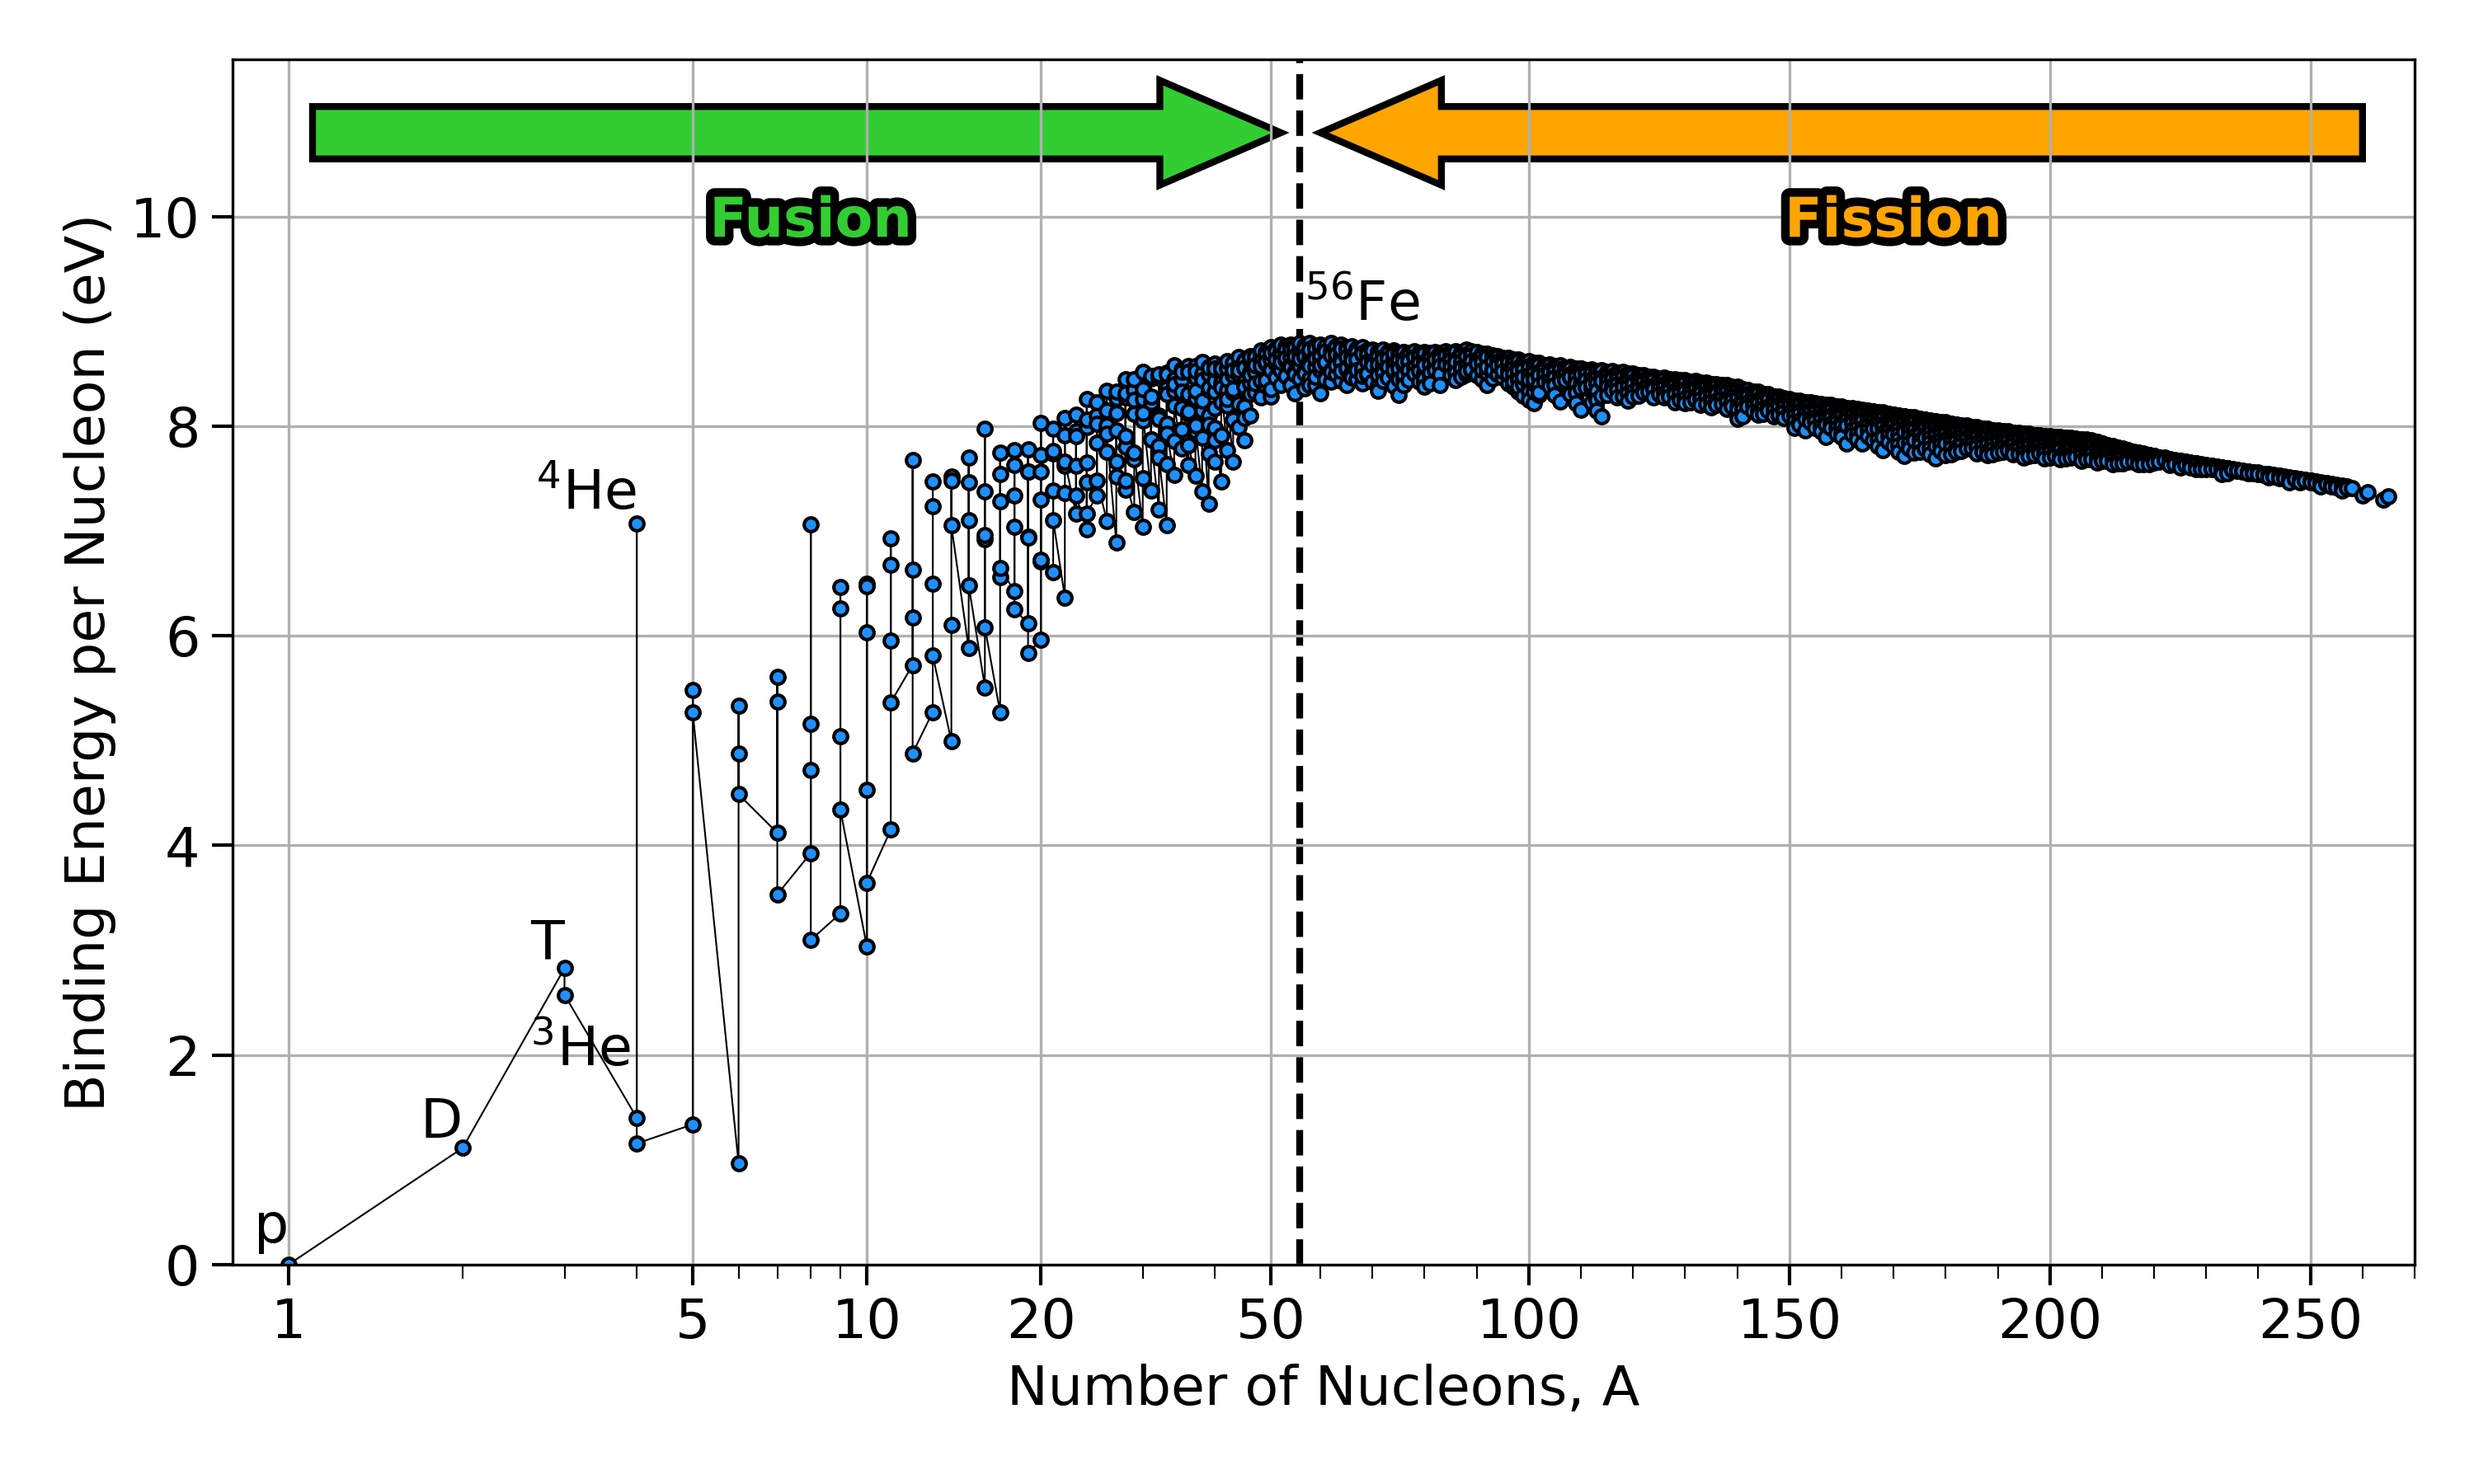
\includegraphics[width=0.9\linewidth]{Introduction/Images/BE_per_nucleon.png}
    \centering
    \caption{Binding energy per nucleon for common nuclear isotopes.
    Binding energy peaks close to iron, therefore energy is released for reactions which increase binding energy.
    ${}^{4}\text{He}$ has a particularly high binding energy and therefore fusion reactions which results in this isotope are strong candidates for fusion energy production.}%
    \label{fig:intro_BEperNucleon}
\end{figure}

\begin{figure}[t!]
    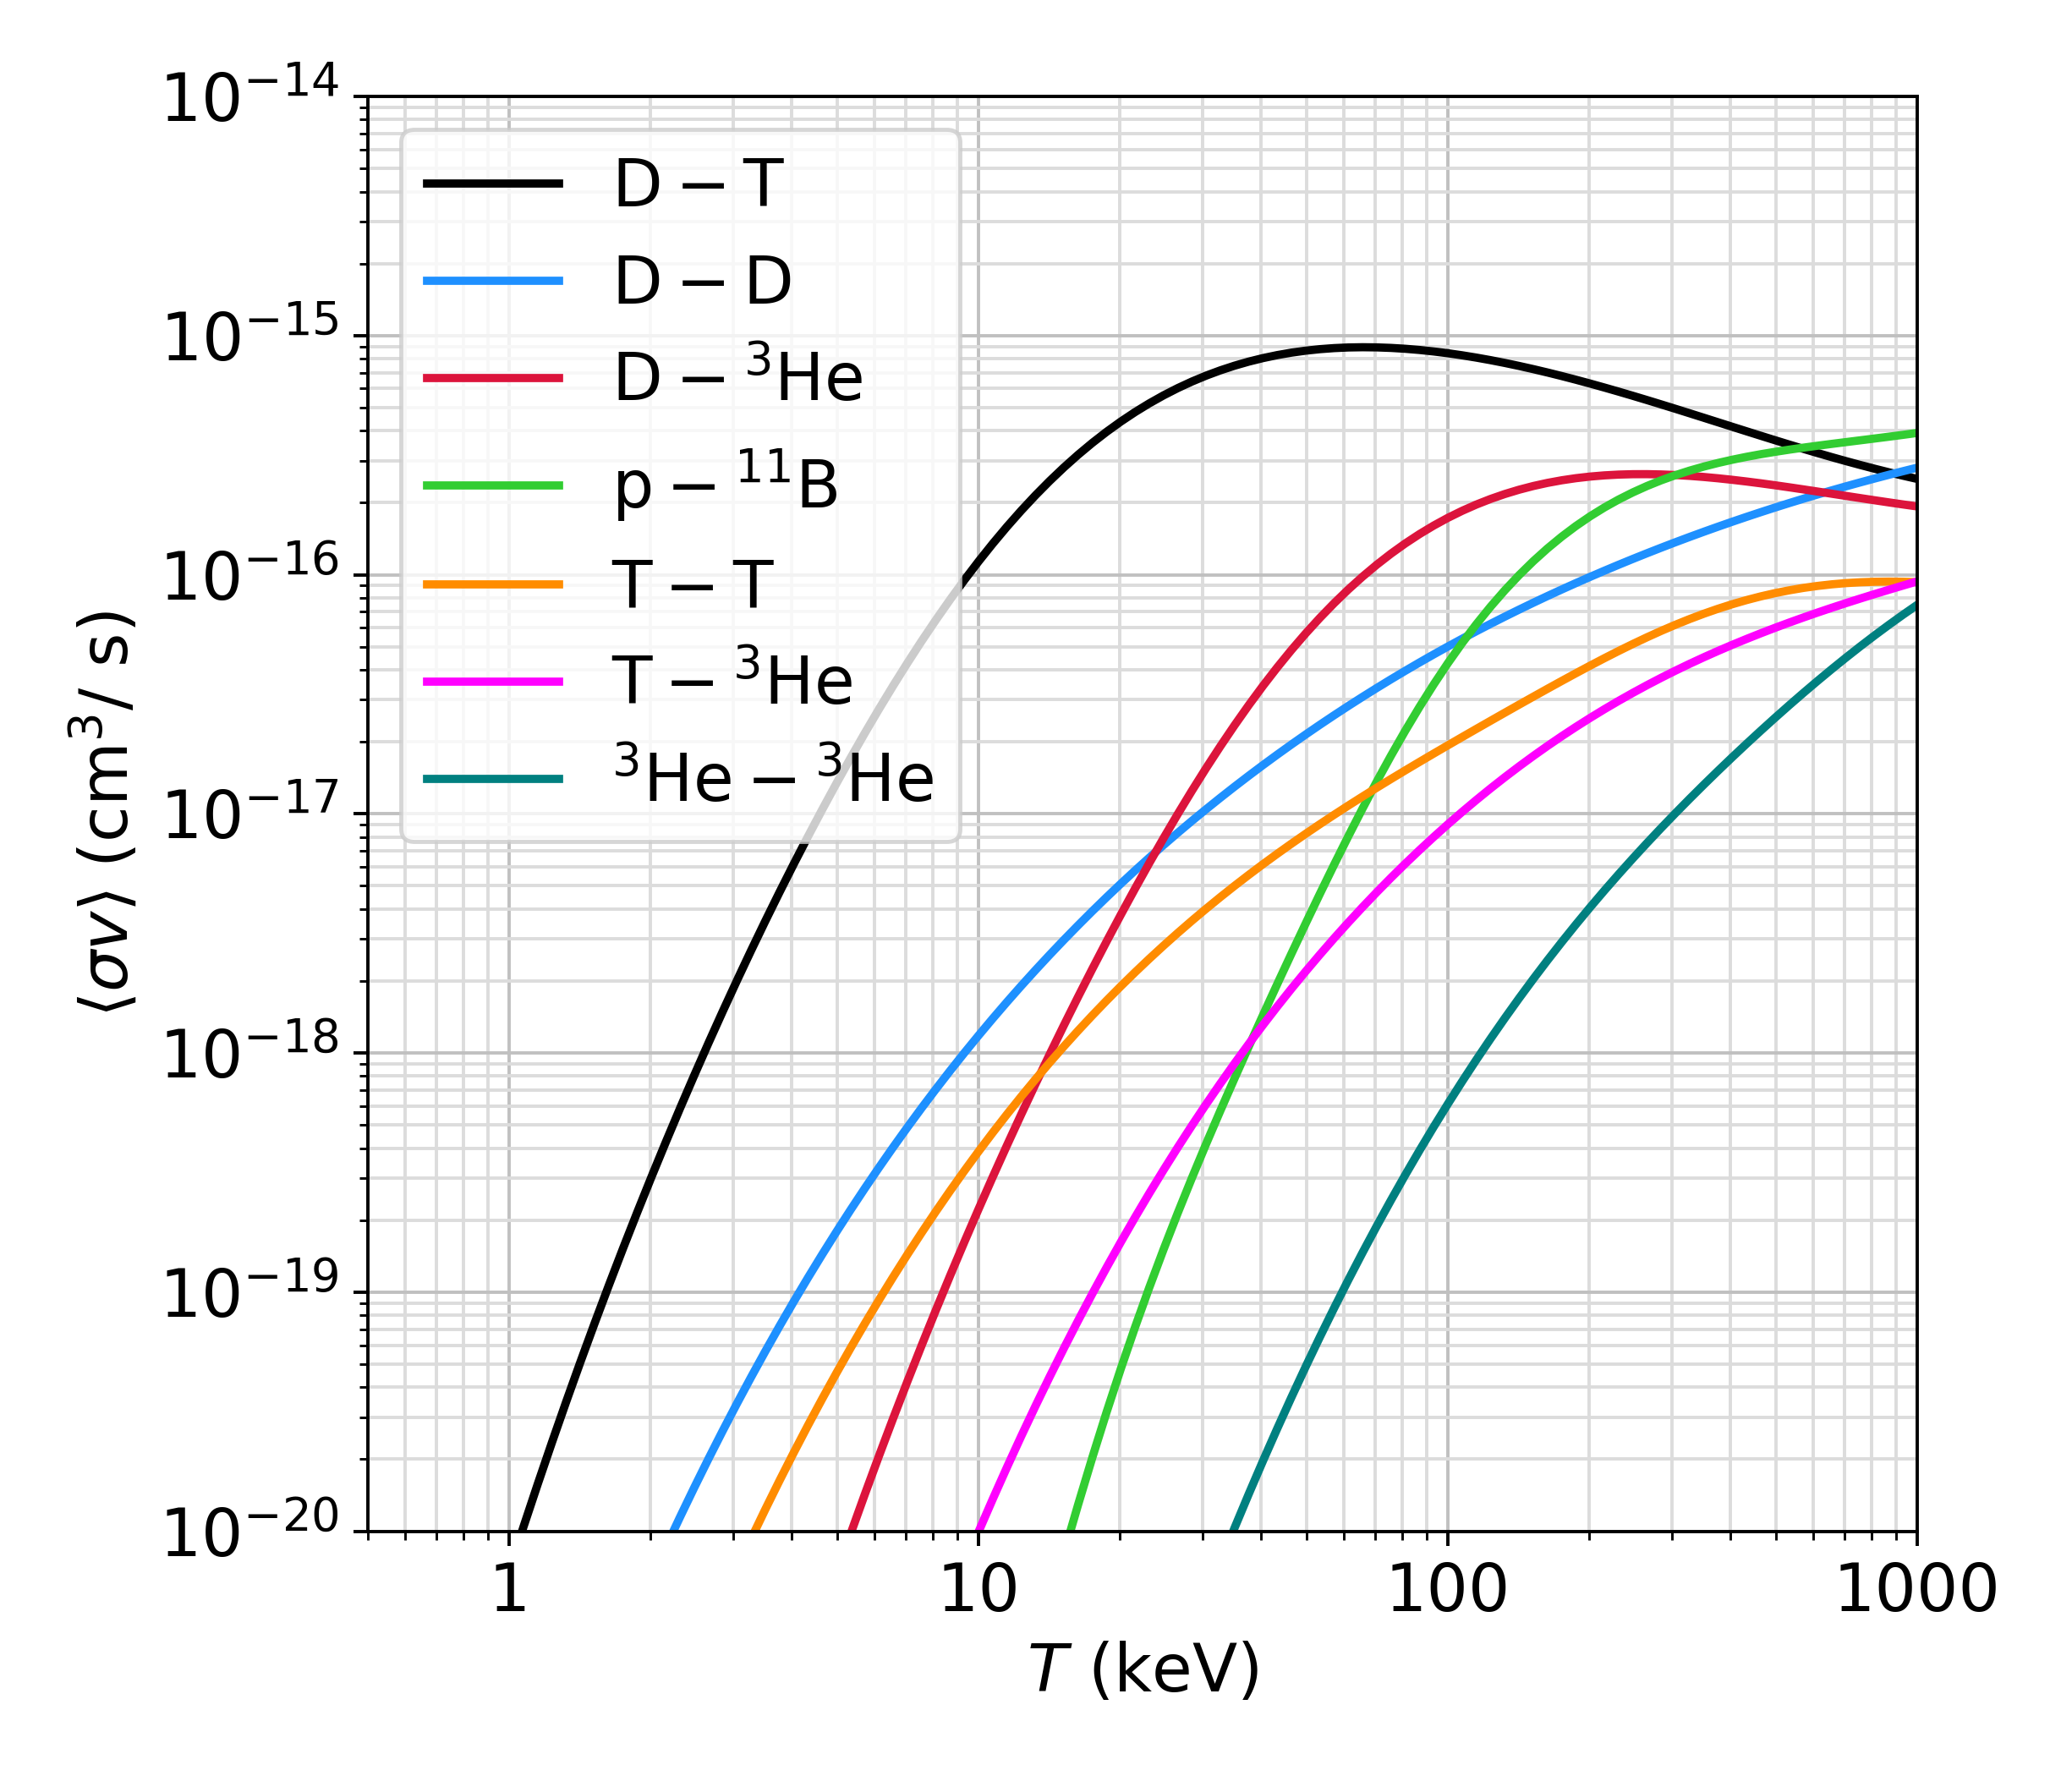
\includegraphics[width=0.6\linewidth]{Introduction/Images/fusion-reactivities.png}
    \centering
    \caption{Averaged reactivities for important fusion reactions.
    The deuterium-tritium reactivity is significantly larger than all other reactions up to $T\sim500\ \text{keV}$.
    Averaged reactivities are obtained from cross-section data, available in the \texttt{ENDF/B-VII.1} library~\cite{chadwick_endf_2011}.
    }%
    \label{fig:intro_reactivities}
\end{figure}

The efficacy of a fusion fuel is dictated by the availability of the reactants, the fusion products, the averaged reactivity of the reactants and the energy released per reaction, $Q$, which is the difference in binding energy between the reactants and products.
Most current, fusion-energy experiments are focussed on demonstrating that fusion power production is possible, thus the choice of fuel is predominantly dictated by the reactivity.
Hydrogen-Hydrogen isotope fusion reactions have much higher reactivities than other elements, because the Coulomb repulsion scales as $Z^2$, thus the Gamow energy, $E_G$ is significantly smaller.
The nuclear physics is particularly favourable for the fusion of deuterium (D) and tritium (T), because there is a nuclear resonance at relatively modest energies for the reaction chain which produces an excited, unstable ${}^5 \text{He}$ nucleus, which subsequently decays to ${}^4\text{He}$ and a neutron~\cite{brown_field_2014}.
Averaged-reactivates of several important fusion reactions, obtained from reaction cross-sections from the \texttt{ENDF/B-VII.1} library~\cite{chadwick_endf_2011}, are plotted in Fig.~\ref{fig:intro_reactivities}.
The D-T reactivity is at least an order of magnitude larger than the other reactions plotted, up to $T\sim100\ \text{keV}$, and it is thus the most commonly used fuel for high-gain fusion experiments.
The reaction proceeds as,
\begin{equation}
    \label{eq:intro_DTreac}
    {}^{2}_{1}\text{D} + {}^{3}_{1}\text{T} \rightarrow \alpha(3.5\ \text{MeV}) + \text{n}(14.1\ \text{MeV}),
\end{equation}
where $\alpha$ is a ${}^{4}_{2}\text{He}$ nucleus, which gains $3.5\ \text{MeV}$, and $\text{n}$ is a neutron, which gains $14.1\ \text{MeV}$ from the fusion energy released, $Q$.
The energy partition is dictated by energy-momentum conservation of the products in the centre of mass frame.
The alpha particles typically couple their energy back into the bulk fuel via Coulomb collisions, which has the effect of raising the fuel temperature and thus further raising the reactivity, for fuel temperatures below $T\sim60\ \text{keV}$.
Neutrons have a much lower reaction cross-section because they are not charged, and thus typically leave the reaction region.
However, in fusion experiments with high density configurations such as \ac{ICF}, their heating of the fuel can also play a significant role~\cite{daughton_influence_2023}.

In order for net energy gain, sufficient energy must be released by fusion to compensate for the energy required to perform the experiment.
This requires a fuel configuration with a combination of high temperatures and densities for a large volumetric reaction rate, that is confined for a period of time, which is sufficient for enough reactions to occur.
The method of confinement for fusion energy experiments has two broad streams: \ac{MCF}, where magnetic fields are used to confine steady-state fusion-plasma over long time-scales, and \ac{ICF}, where dense fusion fuel is assembled for a short time period and `confined' by its own inertia.
The work conducted in this thesis is of relevance to \ac{ICF} schemes, specifically those in which the plasma is produced by laser irradiation.

%###############################################################################################################################
%###############################################################################################################################
%###############################################################################################################################
\section{Inertial Confinement Fusion}%
\label{sec:intro_ICF}

In the 1950s and 60s, the first devices were built which demonstrated stimulated emission of microwave~\cite{schawlow_infrared_1958} and optical~\cite{maiman_stimulated_1960} light.
The optical-wavelength lasers were quickly recognised as an ideal driver for a far smaller and therefore less destructive thermonuclear device than was used in warheads, which could thus be used for fusion energy generation~\cite{nuckolls_early_1998}.
Much of the research was declassified and subsequently published in a 1972 article by Nuckolls \textit{et al.} in 1972~\cite{nuckolls_laser_1972}.
In these \ac{ICF} experiments, the high temperatures and densities required to initiate an appreciable number of fusion reactions are maintained over a short timescale, which is set by the inertia of the fuel configuration, before the fuel disassembles due to large pressure gradients.
The required fuel density is typically achieved by an implosion process.
High temperatures are typically obtained either from the conversion to internal energy of the implosion kinetic energy, which is the central hotspot ignition variant, described in Sec.~\ref{sec:intro_centralhotspot}, or via an external heating source, as described in Sec.~\ref{sec:intro_icf_alt}.
Before describing these schemes in more detail however, necessary criterion for energy gain conditions shall be discussed, which are agnostic of how the fusion fuel is assembled and dictate the plasma conditions which must be achieved.

%################################################################################
%################################################################################
\subsection{Ignition Requirements}%
\label{sec:intro_icf_ignition}

The point at which alpha heating becomes the dominant term in the power balance of the fusion fuel is termed `ignition' and it is a necessary condition for high gain \ac{ICF} experiments.
Ignition necessitates that the plasma is confined for a sufficiently long period of time, for an appreciable number of fusion reactions to occur, raising the fuel temperatures and reactivities, which results in a propagating burn wave.
Estimates for the required plasma conditions which must be achieved for this to occur, can be estimated by considering the timescales of confinement and fusion.
Initially, a uniform ion number density $n_i$ and temperature $T$, spherical fuel assembly, with outer radius $R$, shall be considered.
The ions have an average mass, $m_i$, such that the mass-density of the fuel, $\rho = m_i n_i$ and the volume of the fuel sphere, $V = 4\pi R^3/3$.
Dimensional considerations give an order of magnitude estimate for the timescale on which fusion reactions occur,
\begin{equation}
    \tau_{\text{fus}} = \frac{1}{n_i \langle \sigma v \rangle},
\end{equation}
where $n_i$ in the ion number density of the plasma.
A radially inward pressure gradient will exist due to the high temperature of the plasma, which will lead to an inward propagating rarefaction wave, disassembling the fuel.
This rarefaction wave will move at the isothermal sound speed, $c_s=\sqrt{2k_{\text{B}T/m_i}}$,\footnote{The factor of 2 in $C-s$ is because the pressure is the sum of contributions from ions and electrons.} from $t=0$, such that its position is given by $r=R-c_s t$.
Therefore, the timescale on which the burning fuel remains un-rarefied and thus confined is,
\begin{align}
    \begin{split}
        \tau_{\text{conf}} &= \int_0^{R/c_s} \frac{ {(R - c_s t)}^3 }{R^3} \ \text{d}t,\\
        &= \frac{R}{4 c_s}.
    \end{split}
\end{align}
The ratio of these timescales,
\begin{equation}
    \frac{\tau_{\text{conf}}}{\tau_{\text{fus}}} = \frac{\langle \sigma v \rangle \rho R}{4 m_i c_s},
\end{equation}
illustrates that, for ignition and hence gain, \ac{ICF} reactions require a large $\rho R$ value, which is typically referred to as the `areal-density'~\cite{fraley_thermonuclear_1974}.

The timescale ratio can be used to derive the `burn-up fraction', which is defined as the ratio of fusion reactions, $N_{\text{fus}} = R_{\text{DT}}V\tau_{\text{conf}}$, to the number of DT pairs, $N_{\text{DT}}=n_i/2$, in the fuel assembly,
\begin{align}
    \label{eq:intro_burn_frac}
    \begin{split}
        \Phi &\equiv \frac{N_{\text{fus}}}{N_{\text{DT}}},\\
        &= \frac{\langle \sigma v \rangle \rho R}{H_{\text{B}}},
    \end{split}
\end{align}
where the `burn-parameter', $H_{\text{B}} \equiv \langle \sigma v \rangle / 8 m_i c_s$ has been defined.
Eq.~\ref{eq:intro_burn_frac} is only valid for $\Phi \ll 1$, because the conversion of DT pairs into non-fusing products has not been considered~\cite{atzeni_physics_2004}.
A modified form of Eq.~\ref{eq:intro_burn_frac}, which approximately accounts for burn-depletion, was derived by Fraley \textit{et al.} in Ref.~\cite{fraley_thermonuclear_1974},
\begin{equation}
    \Phi = \frac{\rho R}{H_{\text{B}} + \rho R}.
\end{equation}
If solid density DT was used, the mass of fuel required to achieve $\Phi=30\%$ of the fuel would be 2.5 kg, which would release the same energy as 50 kilotons of TNT~\cite{crilly_simulation_2020}.
In order to harness the released fusion energy without destroying the surrounding infrastructure, a smaller mass is required, which necessitates compression of the fuel to achieve the $\rho R$ constraint.
A pellet containing $1\ \text{mg}$, compressed to densities $\mathcal{O}(10^3)$ times solid density, could release $100\ \text{MJ}$ of fusion energy at $\Phi=30\%$.
Spherical compression is optimal because the fuel compresses in three dimensions.
This minimises the convergence ratio, $CR = R_{\text{init}}/R_{\text{final}}$, which increases the tolerance to a given amplitude of perturbation.

%################################################################################
%################################################################################
\subsection{Central Hotspot Ignition}%
\label{sec:intro_centralhotspot}

\begin{figure}[t!]
    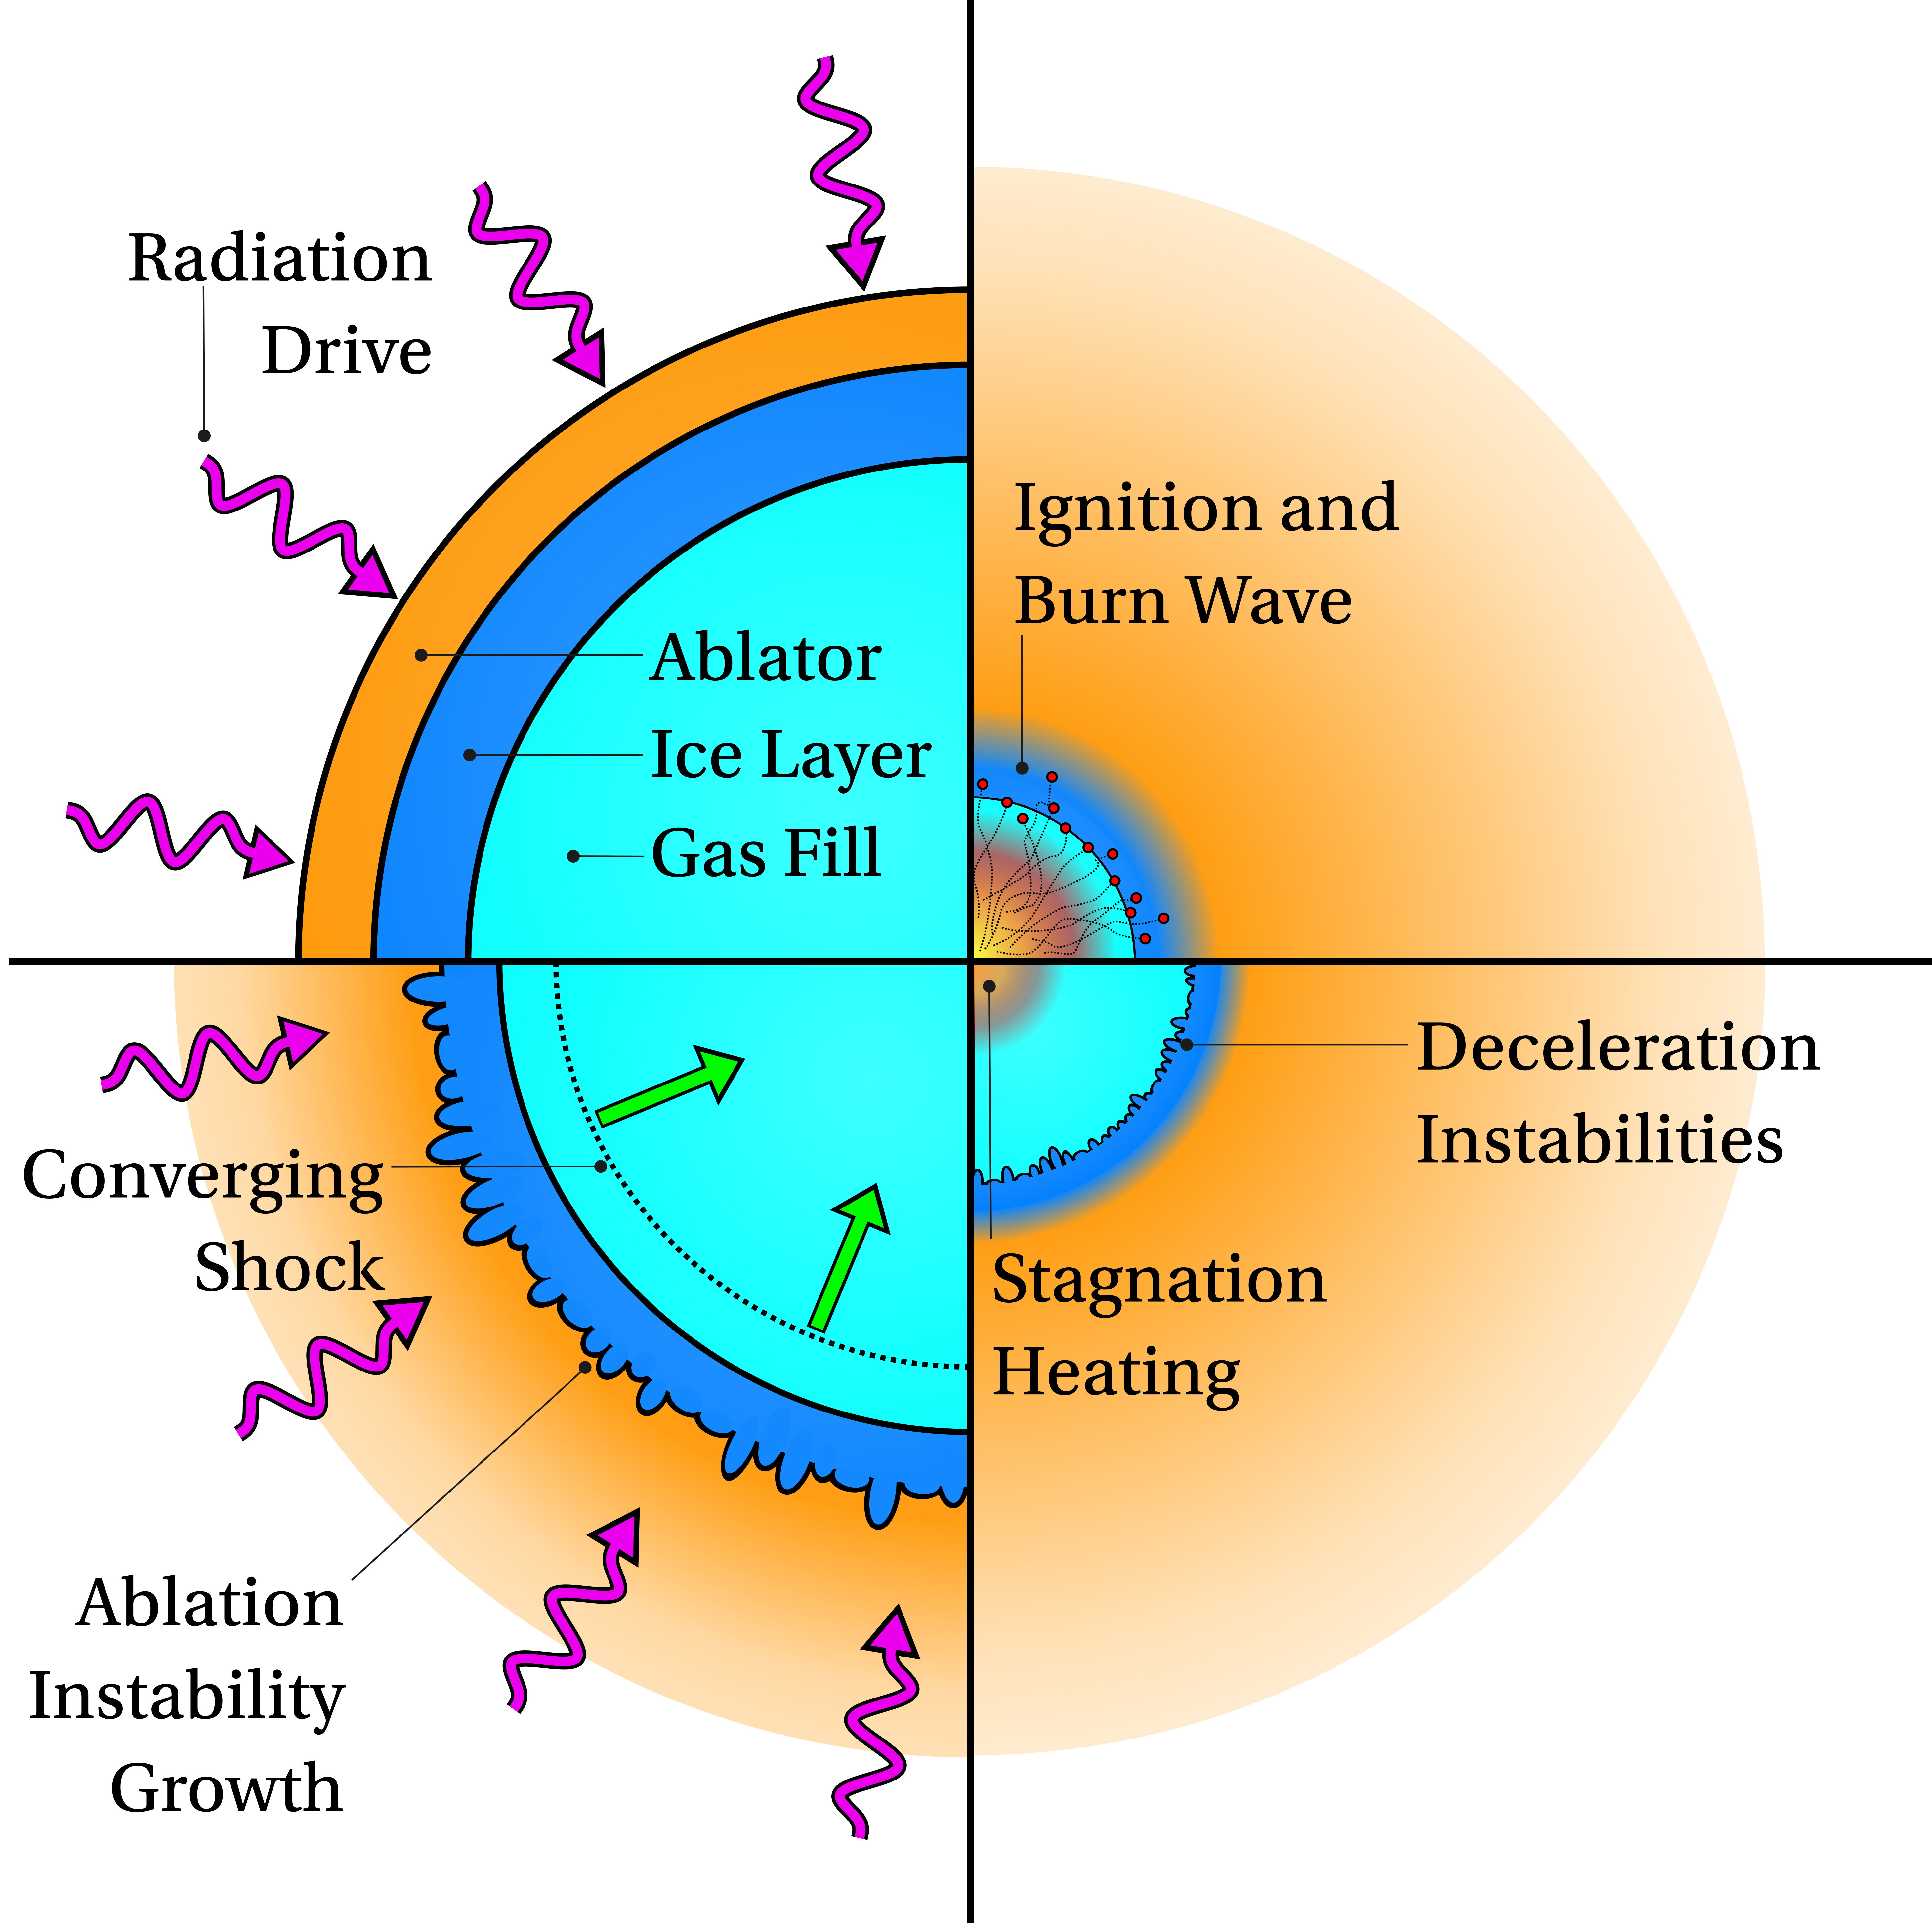
\includegraphics[width=0.7\linewidth]{Introduction/Images/hotspot ignition white.png}
    \centering
    \caption{Four key Stages of the central hotspot ignition \ac{ICF} concept.
    The chronological order of the diagram is top-left, bottom-left, bottom-right and then top-right quadrants, which display the initial configuration, implosion, stagnation and burn propagation stages respectively.
    }%
    \label{fig:intro_hotspot}
\end{figure}

Increasing fuel mass requires larger and larger driver energy to heat to the required fusion temperatures, $T\sim5\ \text{keV}$.
This necessitates larger and more expensive drivers, limiting both the upfront driver cost and potential target gain.
Therefore, schemes which can minimise the driver energy required to ignite a given fuel mass are more practical for current experiments and future power plants.
The `central hotspot ignition' scheme is one such target configuration, where the target is isentropically compressed by carefully constructed pulse shapes, such that it maintains a cold dense fuel shell which implodes inward.
Only a small mass of central fuel is heated to the required fusion temperatures.
The energy required for this heating is provided from implosion kinetic energy of the dense shell.
Fig.~\ref{fig:intro_hotspot} shows a schematic representation of a central hotspot ignition implosion at 4 important stages.
The top left quadrant shows the initial, spherical target configuration, which is comprised of an outer ablator, a solid DT ice layer and an inner DT gas fill.
Choice of ablator material is driven by a number of considerations, including mass ablation rate, minimisation of instability growth, radiation coupling and ease of manufacturing~\cite{lafon_directdriveignition_2015,kline_first_2016,hu_laserdirectdrive_2023,casey_performance_2015}.
Cryogenic temperatures are required to form the ice layer from the DT fuel.
The driver should, ideally, uniformly irradiate the outer surface to maintain the optimal spherical compression and to minimise instabilities growth.
Specific radiation drives shall be discussed in Sec.~\ref{sec:intro_mainexperiments}, but for now, the scheme shall be discussed, while remaining agnostic of the driver.

The bottom left quadrant of Fig.~\ref{fig:intro_hotspot} shows the implosion phase of the scheme.
As the radiation from the driver heats the outer layer of the ablator, it heats up and expands radially outward, which imparts a rocket force on the interior target, propelling it inward.
A low density gas fill is used to make compression of the target easier such that high convergence ratios can be achieved.
Greatest convergence can be achieved if the pressure of the gas fill is minimised and thus high-gain \ac{ICF} targets aim to limit `preheat' of the interior gas fill ahead of the shock.
For example, a poorly pulse-shaped driver will lead to undesired shock heating of the interior fuel ahead of the converging shell, which raises its pressure and thus limits compressibility.
Assuming perfectly spherical targets and driver radiation, isentropic pulses maximise the target gains, which are designed to limit shock preheating of the gas-fill.
In reality, target defects and short wavelength perturbations in the driver radiation seed the \ac{RTI} on the ablation surface, which can grow due to the misaligned density and pressure gradients.
Realistic pulse shapes often slightly preheat the target, which increases stability to hydrodynamic instability growth~\cite{goncharov_improved_2003,hurricane_highfoot_2014}.
The preheat and thus stability of the design, is typically parameterised by the `adiabat' parameter,
\begin{equation}
    \label{eq:intro_adiabat}
    \alpha = \frac{P_{\text{shell}}}{P_{\text{F}}},
\end{equation}
where $P_{\text{shell}}$ is the pressure of the DT shell and $P_{\text{F}}$ is the Fermi degenerate pressure, \textit{i.e.} truly isentropic compression of a $T\sim0\ \text{K}$ fuel has $\alpha=1$.
Higher adiabat designs are more stable, and the parameter is set in each shot by launching a weak shock through the capsule before the main pulse.

The stagnation phase of the implosion is shown in the bottom right quadrant of Fig.~\ref{fig:intro_hotspot}.
As the remaining relatively cold and dense shell converges on the axis, $P\text{d}V$ heating raises the temperature of the compressed interior gas fill.
If the implosion velocity is sufficient, this piston heating of the fuel results is fusion relevant temperatures.
The deceleration phase is also hydrodynamically unstable, because the high pressure, low density interior pushes on the high density, low pressure shell, which results in further \ac{RTI} growth.
Long wavelength perturbations to the radiation drive result in unstagnated kinetic energy in the hotspot, limiting maximum achievable temperatures~\cite{gatujohnson_impact_2018}.
Short wavelength perturbations from the \ac{RTI}, can introduce high-Z ablator material to the hotspot which enhances radiative losses, and if sufficiently large amplitude can puncture the shell, severely degrading confinement~\cite{smalyuk_review_2020}.

The upper-right quadrant of Fig.~\ref{fig:intro_hotspot} shows the final, ignition and burn propagation phase of the design.
If the density and temperature of the fuel hotspot are sufficient, then fusion reactions begin to occur, generating energetic alpha fusion products.
For sufficiently high areal density shells, the alpha particles deposit their energy in the dense fuel shell, raising its temperature and introducing further fusion fuel to the burn process.
This leads to ignition, if the confinement holds the fuel together for a sufficiently long period.

%################################################################################
%################################################################################
\subsection{Alternative Ignition Approaches}%
\label{sec:intro_icf_alt}

In the central hotspot ignition scheme, the energy required to heat the fuel to fusion temperatures is supplied by the kinetic energy of the imploding shell.
The high shell velocities required to result in hotspot fusion temperatures is $\sim300\ \text{km/s}$ and results in significant instability growth.
Alternative schemes exist, namely the shock- and fast-ignition variants, where the required shell density is obtained via a much slower implosion process, limiting instability growth.
Temperatures are then achieved by applying a heating source, separate from the implosion dynamics.
For shock ignition, the driver pulse shape is sharply ramped up at the end of the pulse, in order to generate a strong, spherically converging shock, heating the fuel to fusion temperatures~\cite{betti_shock_2007,perkins_shock_2009}.
The main issue with this scheme for laser-driven \ac{ICF}, has been questions over laser coupling at the high intensities required to generate the ignitor shock.
At high laser intensities, a mostly deleterious class of laser-plasma interaction known as \ac{LPIs} dominate.
\ac{LPIs} are introduced in detail Sec.~\ref{sec:intro_LPIs}.
Recent work has explored the possibility of augmenting the laser pulse shape to add a dip in power, prior to the ignitor pulse rise, which aids in shock generation and thus limits the intensities required~\cite{scott_shockaugmented_2022}.

Fast-ignition is an alternative concept which utilises an external ignitor-beam, of charged particles, to provide the hotspot heating~\cite{tabak_ignition_1994}.
Scientific research related to this scheme include studying how the high energy charged particles are generated via ultra-intense laser interactions, and they can be focused and couple their energy to the fuel~\cite{jarrott_visualizing_2016,gong_direct_2019}.
The overall complexity of many of proposed driver and target configurations would also likely have to be reduced, in order to make \ac{IFE} relevant targets.

All the ignition concepts introduced so far focus on igniting a small central mass, which then initiates a propagating burn wave into surrounding fuel.
The volume-ignition variant, instead proposes igniting the entire fuel volume simultaneously~\cite{khoda-bakhsh_advanced_1992,molvig_low_2016}.
This is achieved by assembling a large, dense fuel mass, kept at a much lower temperature than the hotspot in other schemes.
A large and dense fuel assembly has minimal radiative losses and can thus ignite at $T\sim1.5\ \text{keV}$, as opposed to the ideal ignition temperature of hotspot schemes, $T=4.3\ \text{keV}$~\cite{atzeni_physics_2004}\footnote{The ideal ignition temperature is the value at which alpha heating balances alpha heating.}.
One issue with this scheme is that significantly more laser energy is required to ignite a given fuel mass, because the entire volume must be brought to ignition conditions at the same time.

%################################################################################
%################################################################################
\subsection{Inertial Fusion Energy Considerations}%
\label{sec:intro_IFE_gain}

\begin{figure}[t!]
    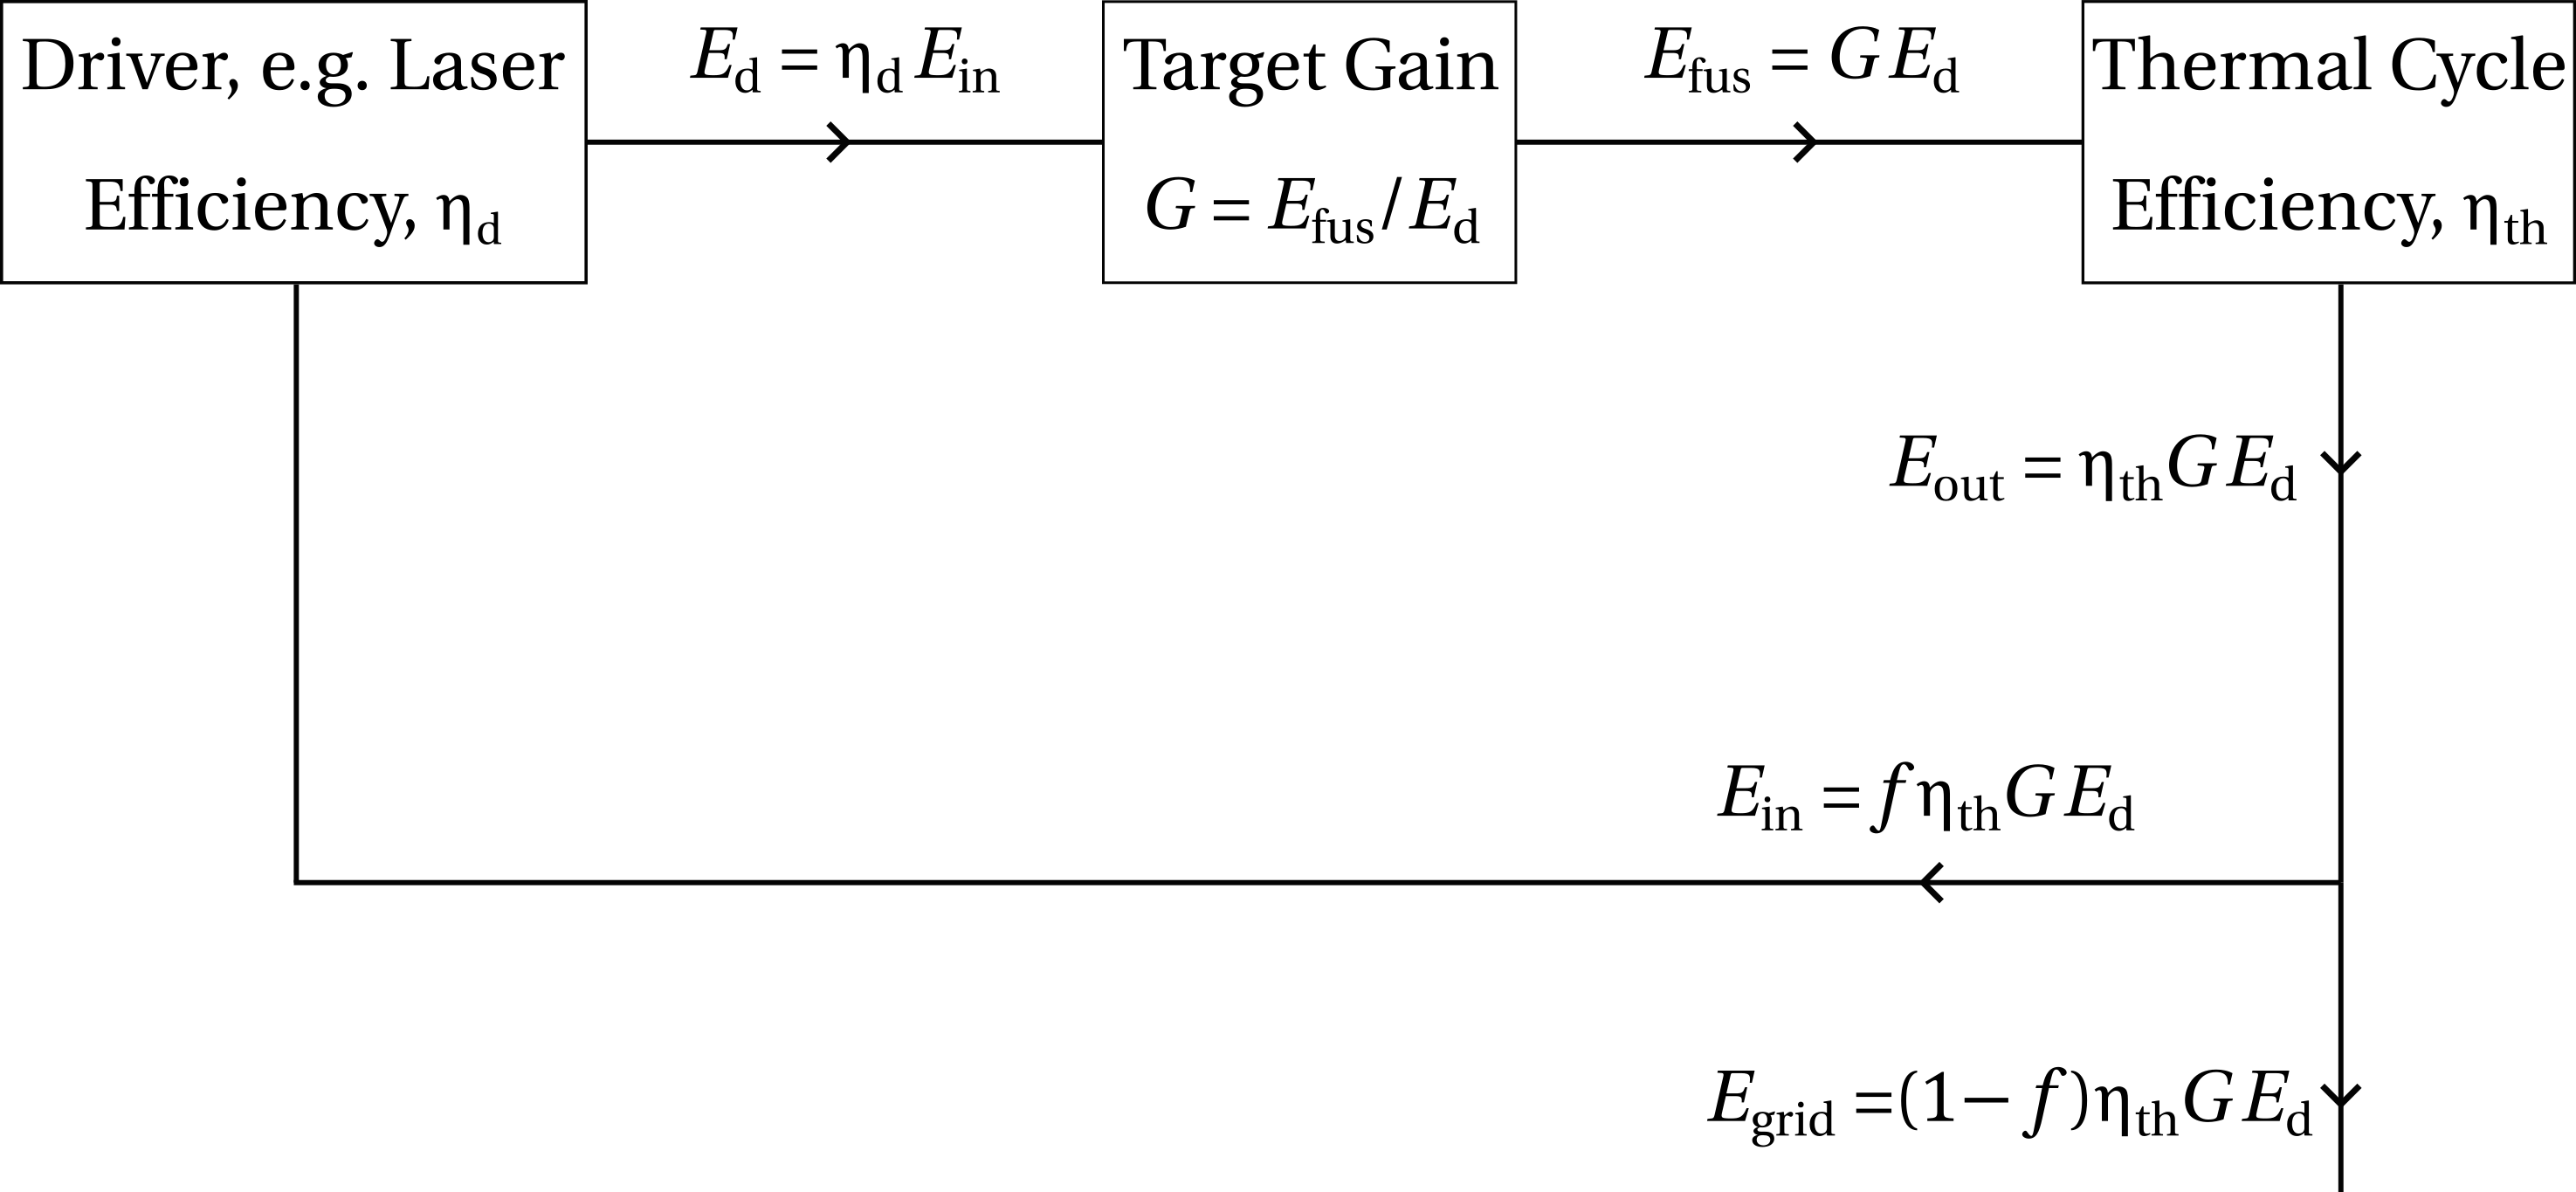
\includegraphics[width=0.8\linewidth]{Introduction/Images/IFE_powerplant.png}
    \centering
    \caption{Energy balance of an \ac{IFE} power plant.
    Based on a similar figure from Ref.~\cite{atzeni_physics_2004}.
    }%
    \label{fig:intro_IFE_energy_balance}
\end{figure}

For a power plant to produce net energy from \ac{ICF} implosions, the energy from each target must of course be greater than the energy to drive the implosion.
In reality, additional inefficiencies in power plants set more stringent constraints on the energy which must be produced.
The energy balance of an \ac{IFE} power plant is shown in Fig.~\ref{fig:intro_IFE_energy_balance}.
A driver, such as the lasers which are considered for the work conducted in this thesis, converts an input energy, $E_{\text{in}}$, to a driver energy, $E_{\text{d}} = \eta_{\text{d}}E_{\text{in}}$, where $\eta_{\text{d}}$ is the energy efficiency of the driver.
The driver energy initiates a fusion reaction, which releases energy $E_{\text{fus}}$, with gain, $G = E_{\text{fus}}/E_{\text{d}}$.
The released fusion energy, for example in the form of energetic neutrons, is converted into thermal energy in an encompassing `blanket', and then into output electrical energy, $E_\text{out}$ by a thermal-cycle (such as steam turbines), with efficiency, $\eta_{\text{th}}$.
Some fraction $f$ of this generated energy is recycled back into the plant to power the driver and the remaining fraction is sent to the grid,
\begin{equation}
    E_{\text{grid}} = (1-f) \eta_{\text{th}} \eta_{\text{d}} G E_{\text{in}},
\end{equation}
with the constraint, $f \eta_{\text{th}} \eta_{\text{d}} G \geq 1$ for net energy production.
Power plants must also produce a sufficiently large volume of energy to be economical.
Therefore, several $\sim100\ \text{MJ}$ reactions must occur each second for a $100\ \text{MW}$ plant, which necessitates a driver that can operate at $\sim10\ \text{Hz}$.

The \ac{DPSSL} concept, could feasibly produce laser energy at $\sim10\ \text{Hz}$ repetition rate, with an efficiency $\eta_d\sim10\%$.
Assuming a thermal cycle efficiency, $\eta_{\text{th}}=40\%$ and a recycled energy fraction, $f=1/4$, this means that a target gain of approximately $G\sim100$ is required for power production.
Additionally, the plant must be economically profitable, thus for a $G=100$ reaction, which releases $E_{\text{fus}} = 100\ \text{MJ} = 28\ \text{kWh}$, the energy sold to the grid would make about £1.50\footnote{The UK April 2024 energy price of £0.25 per $\text{kWh}$ was used.}.
Therefore, targets must cost approximately £0.10, which limits the tolerable manufacturing complexity.
\ac{IFE} target concepts exist, which could feasibly be mass-produced for an acceptable cost, for example initially uniform density liquid spheres, known as `dynamic shell' targets~\cite{goncharov_novel_2020,igumenshchev_proofprinciple_2023}.

%###############################################################################################################################
%###############################################################################################################################
%###############################################################################################################################
\section{Current Experiments/ Main Approaches}%
\label{sec:intro_mainexperiments}

In Sec.~\ref{sec:intro_ICF}, the basic principles of \ac{ICF} were introduced without specifying the driver technology.
Although heavy ion beams have been proposed as a driver technology~\cite{metzler_target_1984}, most current research focusses on the direct-drive and indirect-drive approaches, which use laser light to directly and indirectly irradiate the target respectively.
For the direct-drive approach, laser are focussed upon the outer surface of the target, whereas in indirect-drive, they illuminate the interior surface of a high-Z material `hohlraum', which generates a thermal bath of x-rays.
The indirect-drive approach was developed in order to relax requirements on laser beam uniformity and sensitivity to hydrodynamic instabilities in direct-drive~\cite{lindl_development_1995}.
Sources of degradation and implosion dynamics are somewhat different in each of these approaches.
Each approach is introduced below, and progress on the main experimental facilities is summarised.

%################################################################################
%################################################################################
\subsection{Indirect-Drive}%
\label{sec:intro_indirect}

\begin{figure}[t!]
    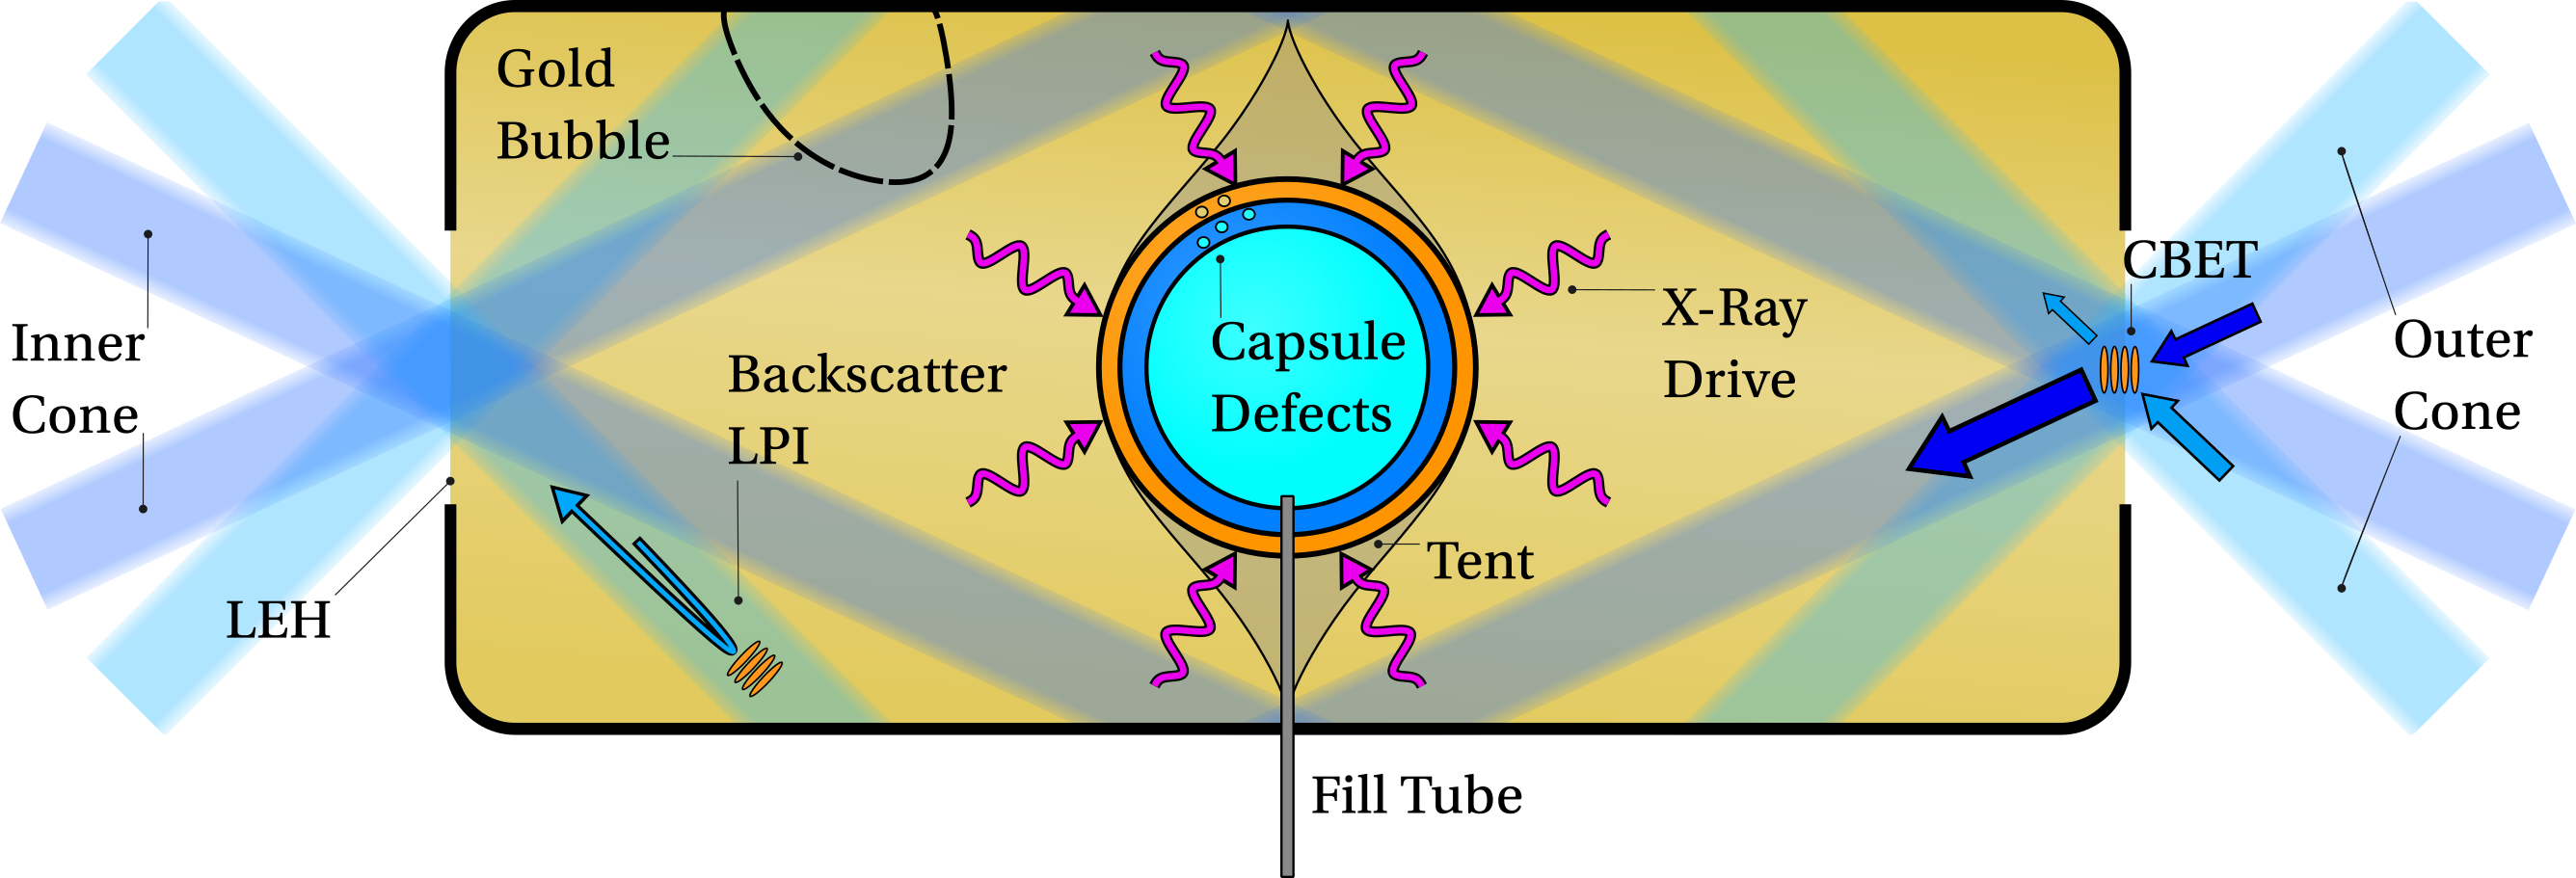
\includegraphics[width=\linewidth]{Introduction/Images/indirect icf white.png}
    \centering
    \caption{Schematic of the indirect-drive approach to \ac{ICF}.
    Laser light, represented as blue transparent rectangles, irradiate the interior of a high-Z (\textit{e.g.} gold) hohlraum, which produces thermal x-rays that drive the capsule implosion.
    A number of important physical effects, typical to indirect-drive experiments, are also illustrated on the diagram.
    }%
    \label{fig:intro_indirect}
\end{figure}

A schematic of an indirect-drive experiment is shown in Fig.~\ref{fig:intro_indirect}.
The \ac{NIF} at the \ac{LLNL} in the United States of America, is the largest \ac{ICF} facility and high power laser system in the world, and it mainly focusses on the indirect-drive approach to \ac{ICF}~\cite{miller_national_2004,spaeth_description_2016}.
The laser system is composed of 192 beams, which are clustered around two poles, so that they can enter the small \ac{LEH} of the hohlraum, as is demonstrated in Fig.~\ref{fig:intro_indirect}.
Approximately $2\ \text{MJ}$ of laser energy can be delivered to the target, usually on a timescale of $10\rightarrow20\ \text{ns}$.
The \ac{LMJ} is a newer facility at \ac{CEA} in France, which is the largest \ac{ICF} experiment outside the United States.
It is also predominantly focussed on the indirect-drive approach and, although currently still in construction, it is intended to have 176 beams that will deliver approximately $1\ \text{MJ}$ of laser energy to the hohlraum~\cite{fleurot_laser_2005}.

The main benefit of the indirect-drive approach is in the uniformity of the driving radiation.
Laser focal spots are instantaneously highly non-uniform, which can seed instabilities and compression is also limited based on the number of available beams.
Conversion of laser light to z-rays in a hohlraum creates a highly uniformly radiation field inside the hohlraum, which has limited short wavelength perturbations to seed \ac{RTI} growth.
Instability growth is therefore mostly seeded from engineering features, such as the tent used to hold the capsule in place, defects in the capsule and surface roughness, and the fill tube used to insert the fuel~\cite{clark_threedimensional_2016}.
A high-Z material such as gold is used for the hohlraum, due to high laser absorption and emissivity.
Longer wavelength modes can be seeded if the laser heating of the hohlraum is asymmetric.
For example, Fig.~\ref{fig:intro_indirect} shows that the hohlraum wall can heat and expand, blocking the `inner-cone' beams which heat the material near the capsule equator.
Filling the hohlraum with a low-Z gas fill\footnote{A low-Z hohlraum fill is used to limit laser absorption.} to limit the `gold bubble' expansion, however, this allows for deleterious \ac{LPIs} to occur, which reflect laser energy back out of the \ac{LEH}~\cite{macgowan_laser_1996}.
Current experiments on the \ac{NIF}, use a relatively low gas fill to reduce backscatter-\ac{LPIs} (specifically \ac{SBS} and \ac{SRS}), and introduce a wavelength shift between the inner and outer cones of laser beams, which allows for a laser-plasma interaction known as \ac{CBET} to transfer power to the outer beams late in the implosion\cite{michel_tuning_2009,moody_multistep_2012,kritcher_energy_2018}.
This compensates for absorption in the expanding gold bubble and can maintain symmetry of the implosion.
The main drawback of the approach to the direct-drive approach is that the conversion of laser light to capsule kinetic energy via the hohlraum, introduces an additional $\sim10\%$ efficiency decrease, limiting the maximum gains that can be achieved.
Increasing the size of the capsule relative to the hohlraum increases the fraction of x-ray energy which is coupled to the target, but can introduce long-wavelength instabilities if made too large by blocking laser propagation.
Direct-drive is thus often considered the preferred scheme for \ac{IFE}.

\begin{figure}[t!]
    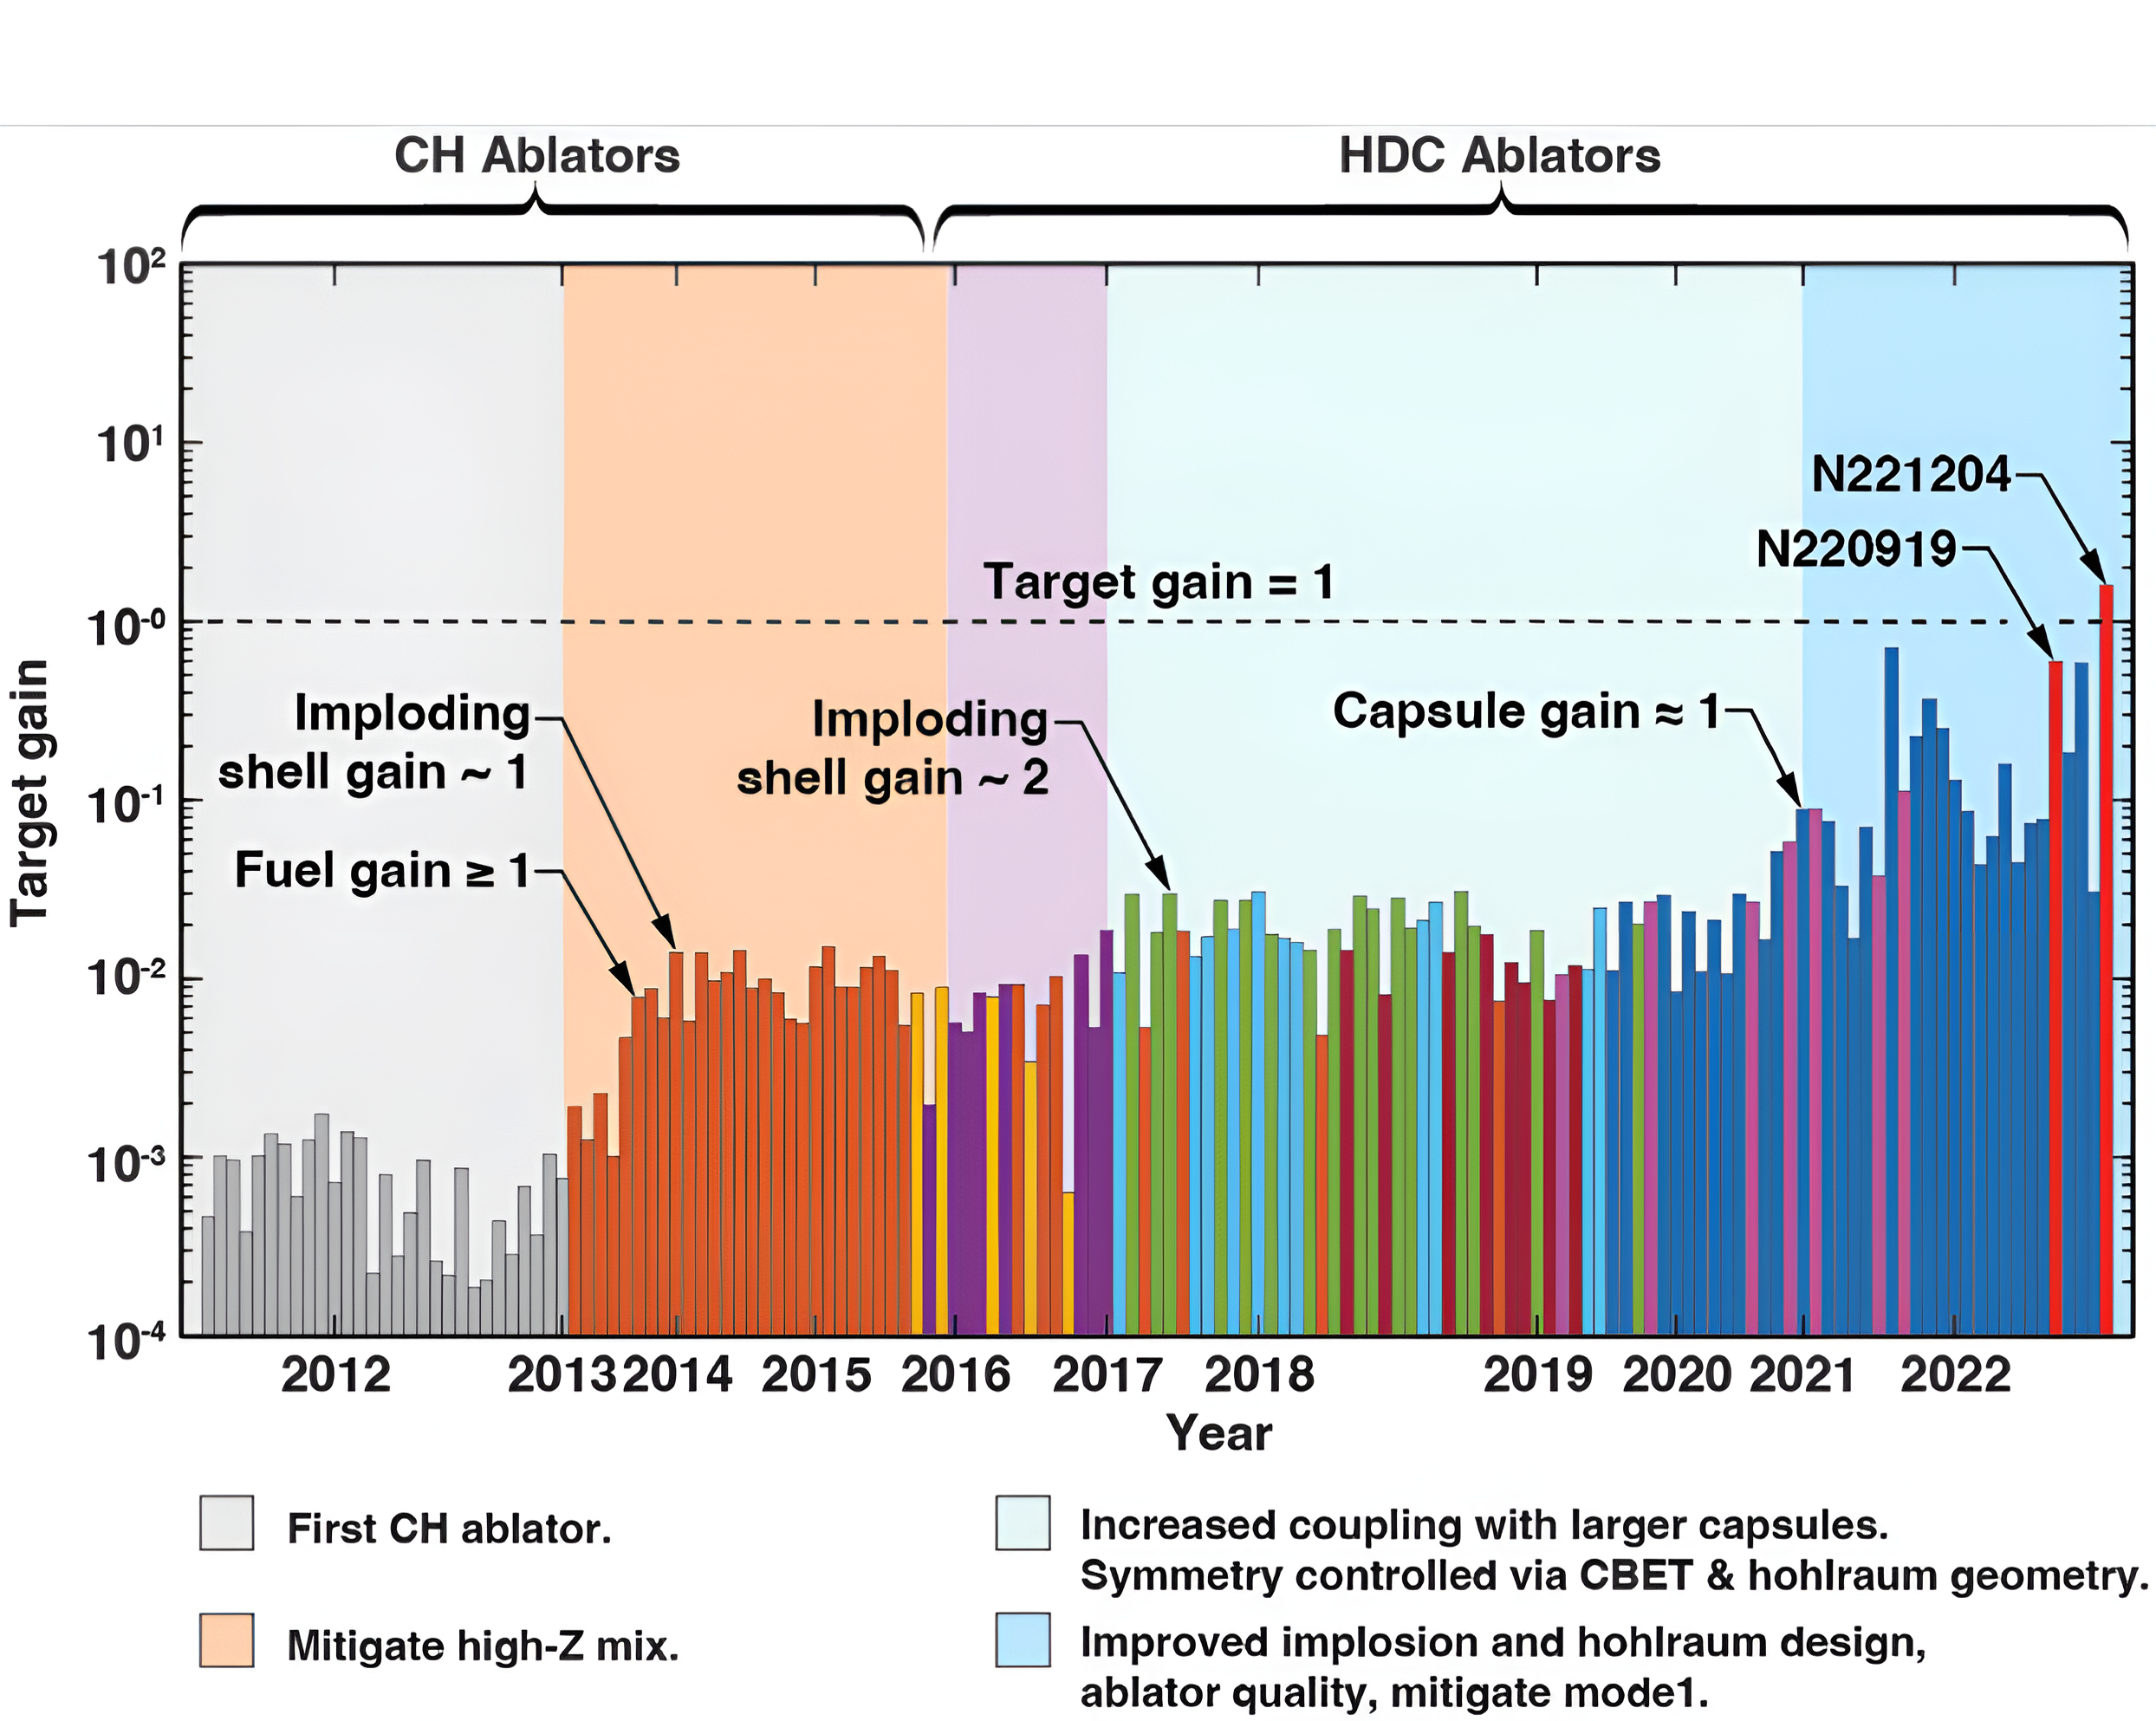
\includegraphics[width=\linewidth]{Introduction/Images/NIF_yields.jpg}
    \centering
    \caption{$G$ plotted against time for indirect-drive \ac{ICF} shots on \ac{NIF}.
    The colour of each bar represents a different implosion design, and the dashed horizontal line represents $G=1$, where the fusion energy produced is equal to the incident laser energy.
    Used under CC BY 4.0 from Ref.~\cite{abu-shawareb_achievement_2024}.
    }%
    \label{fig:intro_nif_yields}
\end{figure}

Although early experiments on the \ac{NIF} dramatically underachieved the main aim of demonstrating ignition, a tremendous amount of progress has been made in recent years \cite{hurricane_physics_2023}.
Fig.~\ref{fig:intro_nif_yields} plots $G$ for indirect-drive \ac{ICF} shots on the \ac{NIF}, up to December 2022~\cite{abu-shawareb_achievement_2024}.
The initial target designs, up to 2013, utilised a low adiabat design, with a plastic (CH) ablator, known as `Low Foot', which proved very sensitive to hydrodynamic instabilities, the results of which are shown in shaded grey in Fig.~\ref{fig:intro_nif_yields}~\cite{lindl_review_2014}.
This led to the subsequent, `High Foot' campaign, where the target was kept similar, but the adiabat of the design was raised to create a more stable implosion, which improved yields, plotted in red~\cite{hurricane_highfoot_2014}.
A new ablator material, \ac{HDC}, was deployed subsequent to this campaign which had a higher density than CH, resulting in improved absorption and thus shorter laser pulses~\cite{mackinnon_highdensity_2014}.
The gas fill-density of the hohlraum was also lowered to reduce the loss of laser energy to backscatter \ac{LPIs}.
The `Hybrid' campaigns made further improvements, by utilising \ac{CBET} to compensate for the loss of symmetry resulting from the gold-bubble expansion in the low-fill hohlraum, using larger capsules to increase coupling efficiency and thicker shells to mitigate instabilities~\cite{zylstra_record_2021}.
Additional improvements were made to capsule quality which minimised sources of instability~\cite{kritcher_design_2024}.
Shots from these campaigns are shown in the light and darker blue in Fig.~\ref{fig:intro_nif_yields} and have led to the achievement of a burning-plasma\footnote{A burning-plasma is defined as plasma where alpha heating is the dominant heating mechanism. This is opposed to ignition, where alpha heating is greater than loss terms.}~\cite{zylstra_burning_2022,kritcher_design_2022} and ignition regimes~\cite{abu-shawareb_lawson_2022}.
This ultimately resulted a shot $G>1$ in December 2022~\cite{abu-shawareb_achievement_2024}.
Although not plotted in Fig.~\ref{fig:intro_nif_yields}, the gain record at the time of writing stands at $G=2.4$~\cite{_nif_}.

%################################################################################
%################################################################################
\subsection{Direct-Drive}%
\label{sec:intro_direct}

\begin{figure}[t!]
    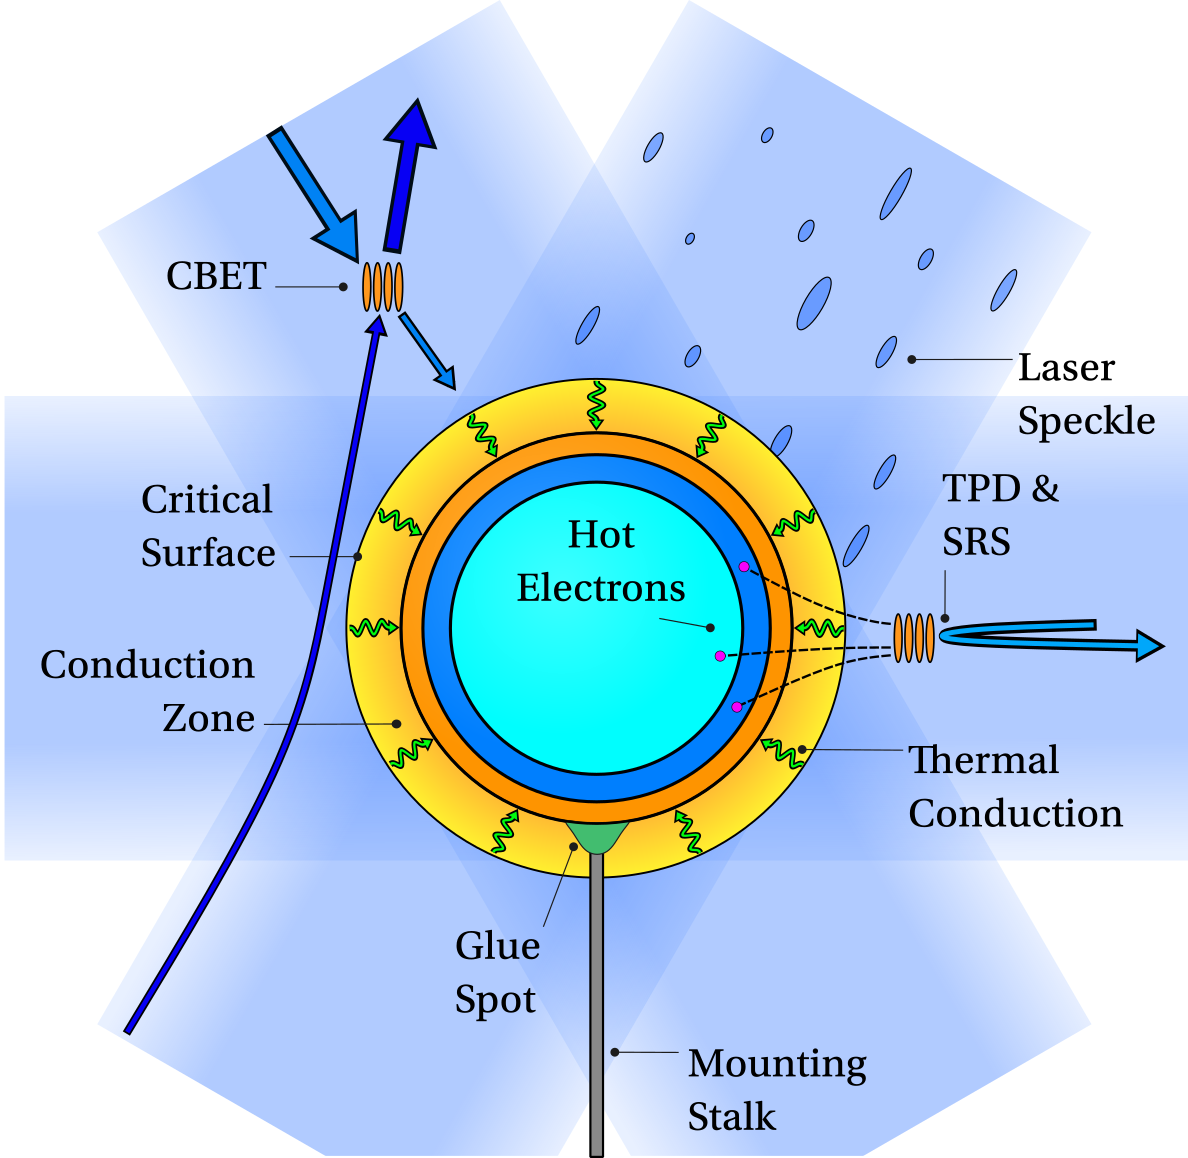
\includegraphics[width=0.7\linewidth]{Introduction/Images/direct icf white.png}
    \centering
    \caption{Schematic of the direct-drive approach to \ac{ICF}.
    Laser light, represented by the transparent, blue rectangles is absorbed outside the critical surface and then transported in to the ablation surface by thermal conduction.
    Speckle from beam smoothing optics leads to short-scale non-uniformity of deposition, known as imprint.
    \ac{LPIs} degrade the performance, both by reflecting light, and by generating hot electrons which pre-heat the fuel.
    }%
    \label{fig:intro_direct}
\end{figure}

A schematic of a direct-drive experiment is shown in Fig.~\ref{fig:intro_direct}.
Although a limited number of direct-drive implosions are performed on the \ac{NIF}, the largest dedicated direct-drive facility in the world is the \textsc{Omega} laser facility at the \ac{LLE} in the United States~\cite{simon_lle_1989,boehly_upgrade_1995}.
Work presented in this thesis is most relevant to direct-drive implosions on this facility.
The \textsc{Omega} laser has a total of 60 beams, arranged to provide approximately symmetric radiation to a spherical target.
In total, beams can deliver approximately $30\ \text{kJ}$ of laser energy to the target, usually in a timescale of $2\rightarrow3\ \text{ns}$.
As previously stated, the high driver efficiencies are desirable for \ac{IFE}, and the relative inefficiency of the hohlraum light to x-ray conversion, means that direct-drive is the assumed driver for a future \ac{IFE} power plant.
As opposed to indirectly-driven \ac{NIF} experiments, where the capsule is held in place by a thin tent attached to the hohlraum, directly-driven \textsc{Omega} targets are glued to a mounting stalk to hold them in place initially.
This can lead to low-mode asymmetries and unstagnated flows in the hotspot, which degrade the performance~\cite{gatujohnson_impact_2020}.

In plasmas, electro-magnetic radiation is absorbed beyond the critical surface, which is the surface interior to which the electron density is sufficiently high, that light of a given wavelength cannot propagate.
For indirect-drive, high frequency x-rays are absorbed close to the ablation surface, whereas for indirect-drive, the longer wavelength laser light has a critical surface which is exterior to the ablation surface.
Thus, energy is absorbed beyond the critical surface, heating this `coronal plasma'\footnote{The term coronal plasma shall be used throughout this thesis to refer to the approximately isothermal, outward flowing, low density plasma blow-off, which is exterior to the critical surface.} to high temperatures.
This absorbed energy is then transported radially inward via thermal conduction in the `conduction-zone', to the higher density, lower temperature ablation surface, as is shown in Fi.g~\ref{fig:intro_direct}.
Non-uniform absorption at the critical surface is partially smoothed by non-radial thermal conduction in this region, which is more efficient for shorter wavelength perturbations.


\begin{figure}[t!]
    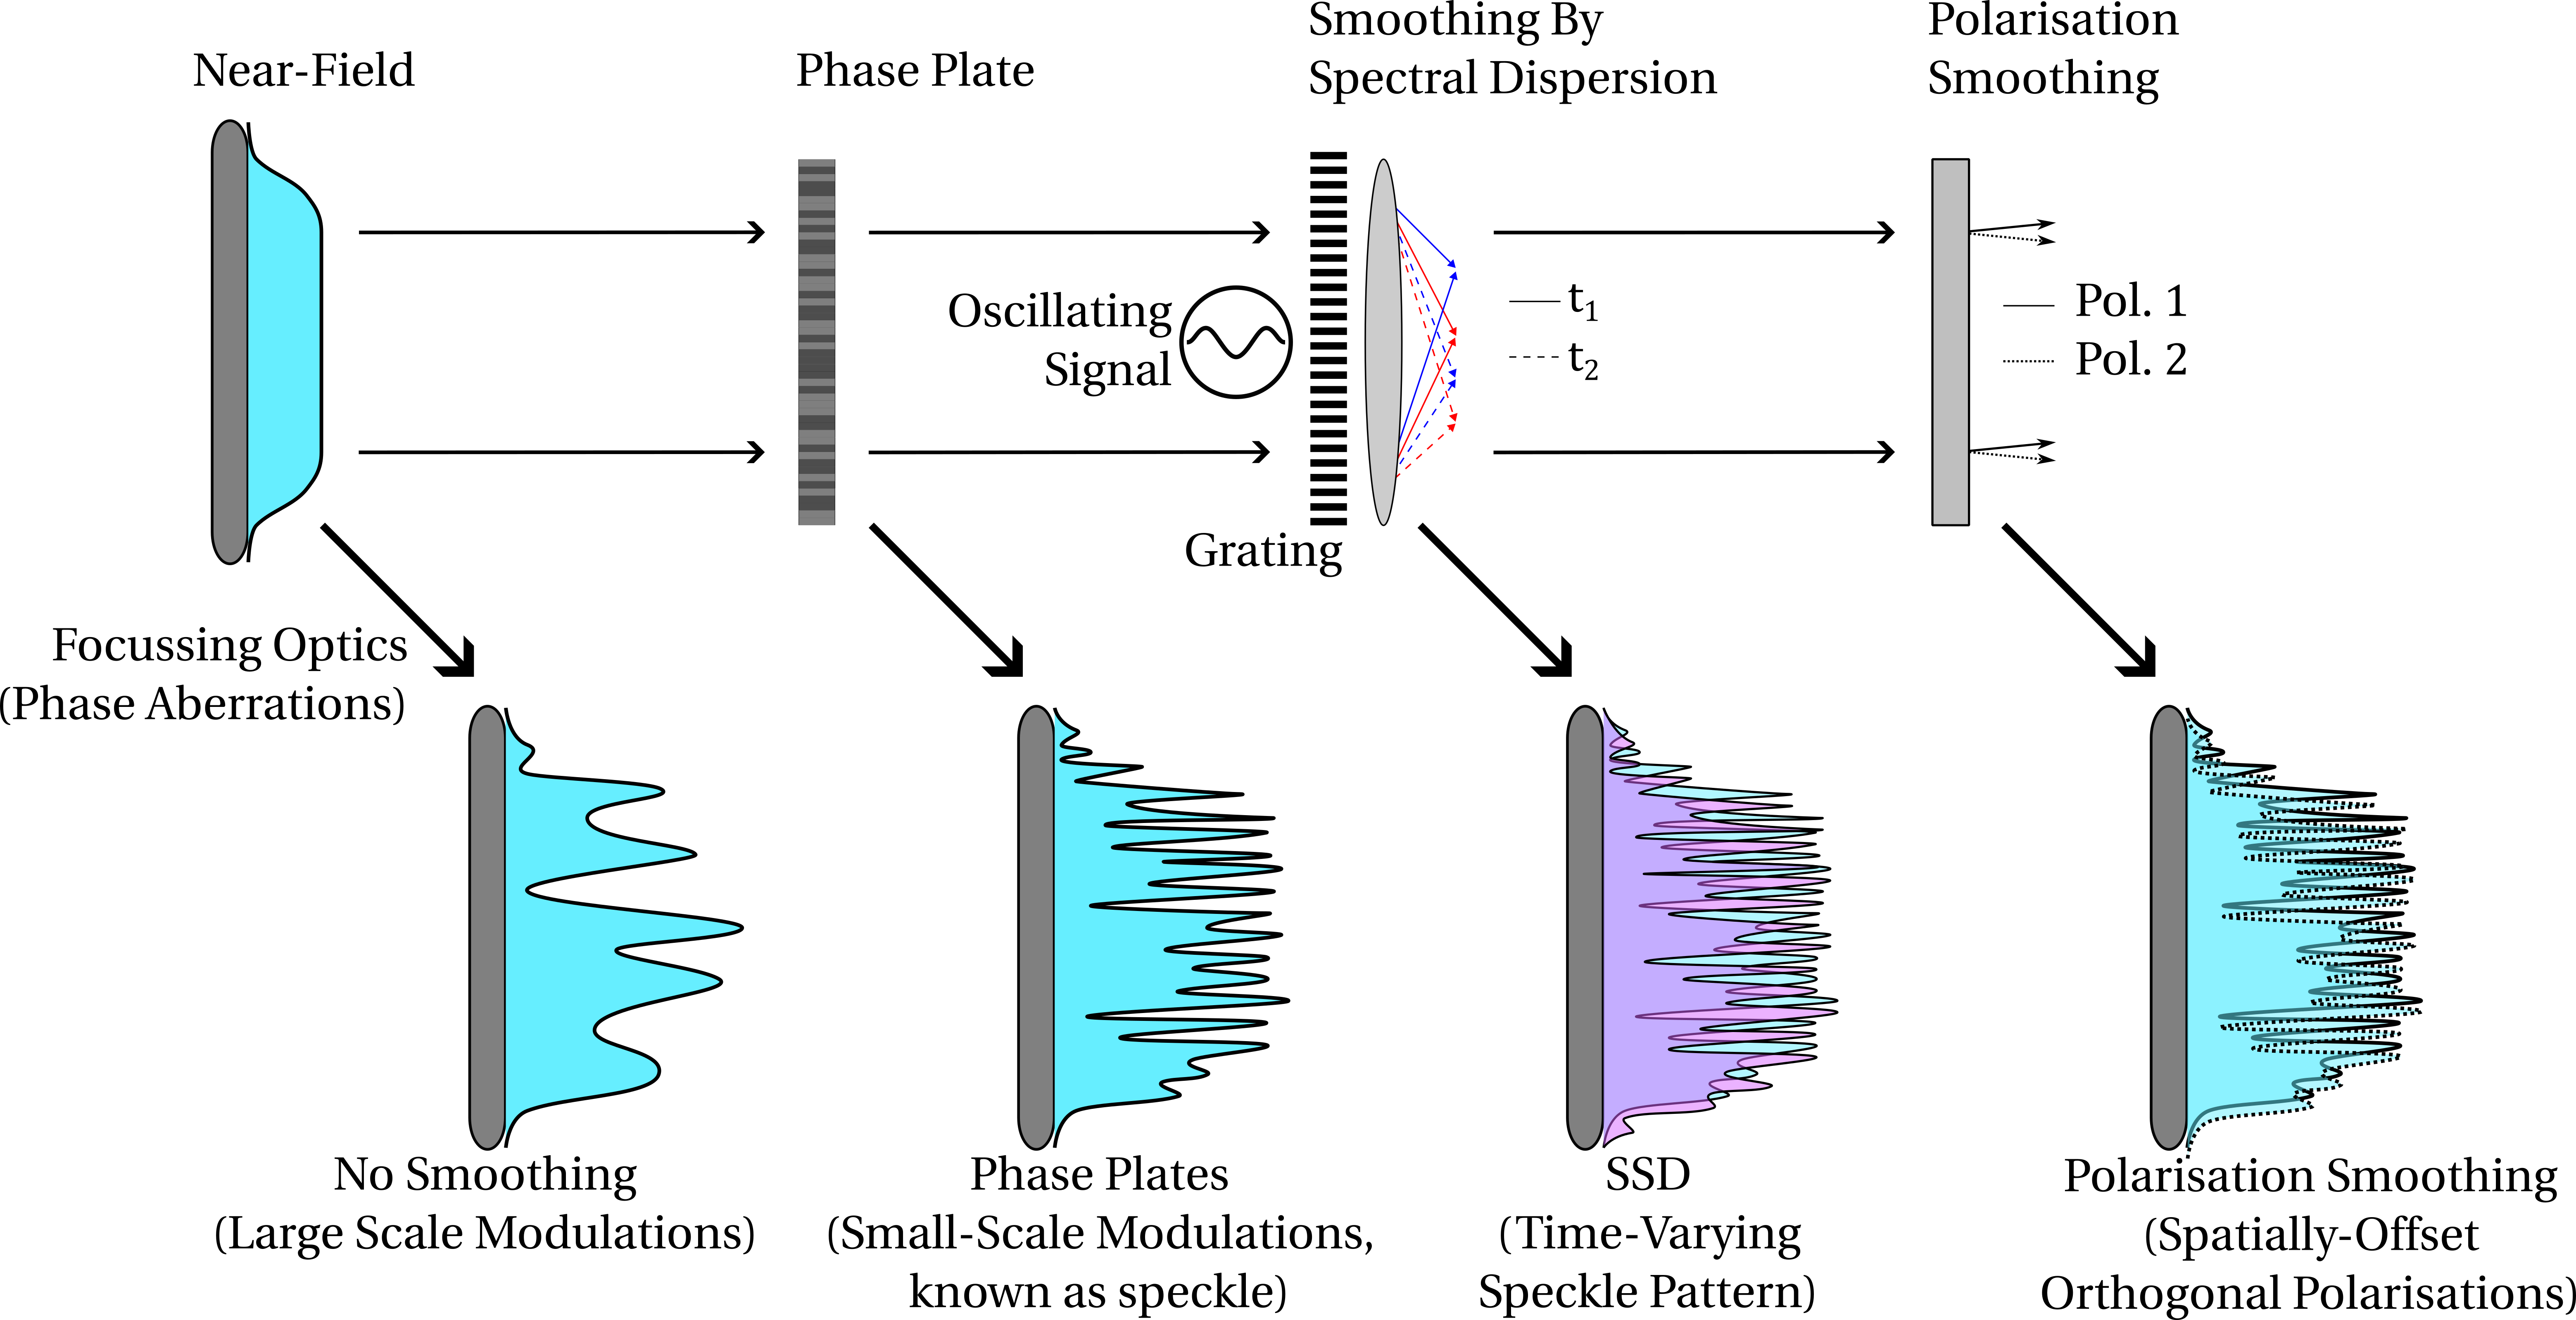
\includegraphics[width=\linewidth]{Introduction/Images/SmoothingOptics.png}
    \centering
    \caption{Schematic of beam smoothing techniques employed on the \textsc{Omega} laser system.
    Phase aberrations can lead to large scale modulations to the far-field intensity profile.
    Phase plates shift the perturbations to shorter scales, which are more efficiently smoother by thermal conduction.
    \ac{SSD} creates a time-varying speckle pattern, which leads to a smooth time-integrated far-field profile.
    Polarisation smoothing splits the beam into orthogonally polarised sub-beams, which do not interfere and thus further reduce non-uniformity.
    }%
    \label{fig:intro_SmoothingOptics}
\end{figure}

Despite this non-radial smoothing in the conduction zone, non-uniformity of the laser drive is a significant difficulty for direct-drive \ac{ICF} implosions.
The number of beams and their widths leads to a `beam-mode' asymmetry, which for \textsc{Omega} has a distinctive Legendre-mode, $\ell=10$ pattern, which can be seen in Fig.~\ref{fig:SOLAS_qpR_IFRIIT_test}.
Focal spots of high power lasers are also often highly non-uniform when so-called `beam-smoothing' techniques are not employed.
As light propagates from the beam port to the far-field, random `phase-aberrations' are picked up by the beam due to distortions in the medium through which it travels, which results in large scale modulations of the focal spot intensity profile.
When the target is illuminated by these modulated beams, significant asymmetry is imparted on the drive, severely limiting the overall performance.
A variety of beam smoothing techniques are thus employed which lead to a significantly more uniform beam profile.
Fig.~\ref{fig:intro_SmoothingOptics} shows a schematic of several important beam smoothing techniques employed by the \textsc{Omega} laser system.
The diagram demonstrates that without beam smoothing, a uniform near-field intensity profile picks up phase aberrations along the laser chain, leading to interference and thus large scale modulations at focus.
Phase plates are an array of small optical elements which offset the phase beam at discrete points in the near-field, acting to shift the scale of modulation in the far-field to a much smaller spatial scale~\cite{kato_random_1984}.
These short-scale modulations are known as `laser-speckle', and are much more easily smoothed in the conduction zone, than the large modulations from beams without smoothing techniques applied.
The static phase plate far-field profile can be further improved by using \ac{SSD}, which creates a temporally varying speckle pattern and thus the time-integrated profile is much smoother.
Fig.~\ref{fig:intro_SmoothingOptics} compactly displays how \ac{SSD} operates, which is to apply a temporally varying bandwidth to the light signal, then pass it through a diffraction grating, such that different wavelengths are dispersed in different directions~\cite{skupsky_improved_1989,hohenberger_optical_2016}.
Finally, Polarisation smoothing is employed on \textsc{Omega}, which works by splitting each beam into two slightly spatially-offset, orthogonally polarised sub-beams.
These sub-beams do not interfere with each other, and thus when added together the root-mean-square intensity variation of the whole beam is improved by a factor $\sqrt{2}$~\cite{tsubakimoto_suppression_1992,boehly_reduction_1999}.

Although the combination of these optics create an intensity spot which is smooth when time-integrated, instantaneously large amplitude, short wavelength perturbations exist.
When an extended plasma corona has formed, these perturbations are effectively smoothed by non-radial thermal conduction in the conduction zone, but early in the implosion, the small amplitude perturbations are deposited close to the ablation surface.
This is known as `laser imprint' and unless mitigated by sufficiently raising the adiabat of the implosion, can break up the shell.
The adiabat is typically set for direct-drive implosion by including a small `picket' pulse in the laser temporal profile, which weakly shocks the shell.
The laser turns off after this picket pulse, leading to an unsupported shock, which decays in amplitude as it travels through the shell, such that only the outer extent of the shell, where the imprint occurs, is on a high adiabat.
Imprint does not occur in indirectly-driven implosion, and thus the highest performing direct-drive experiments normally have much higher adiabats.

\begin{figure}[t!]
    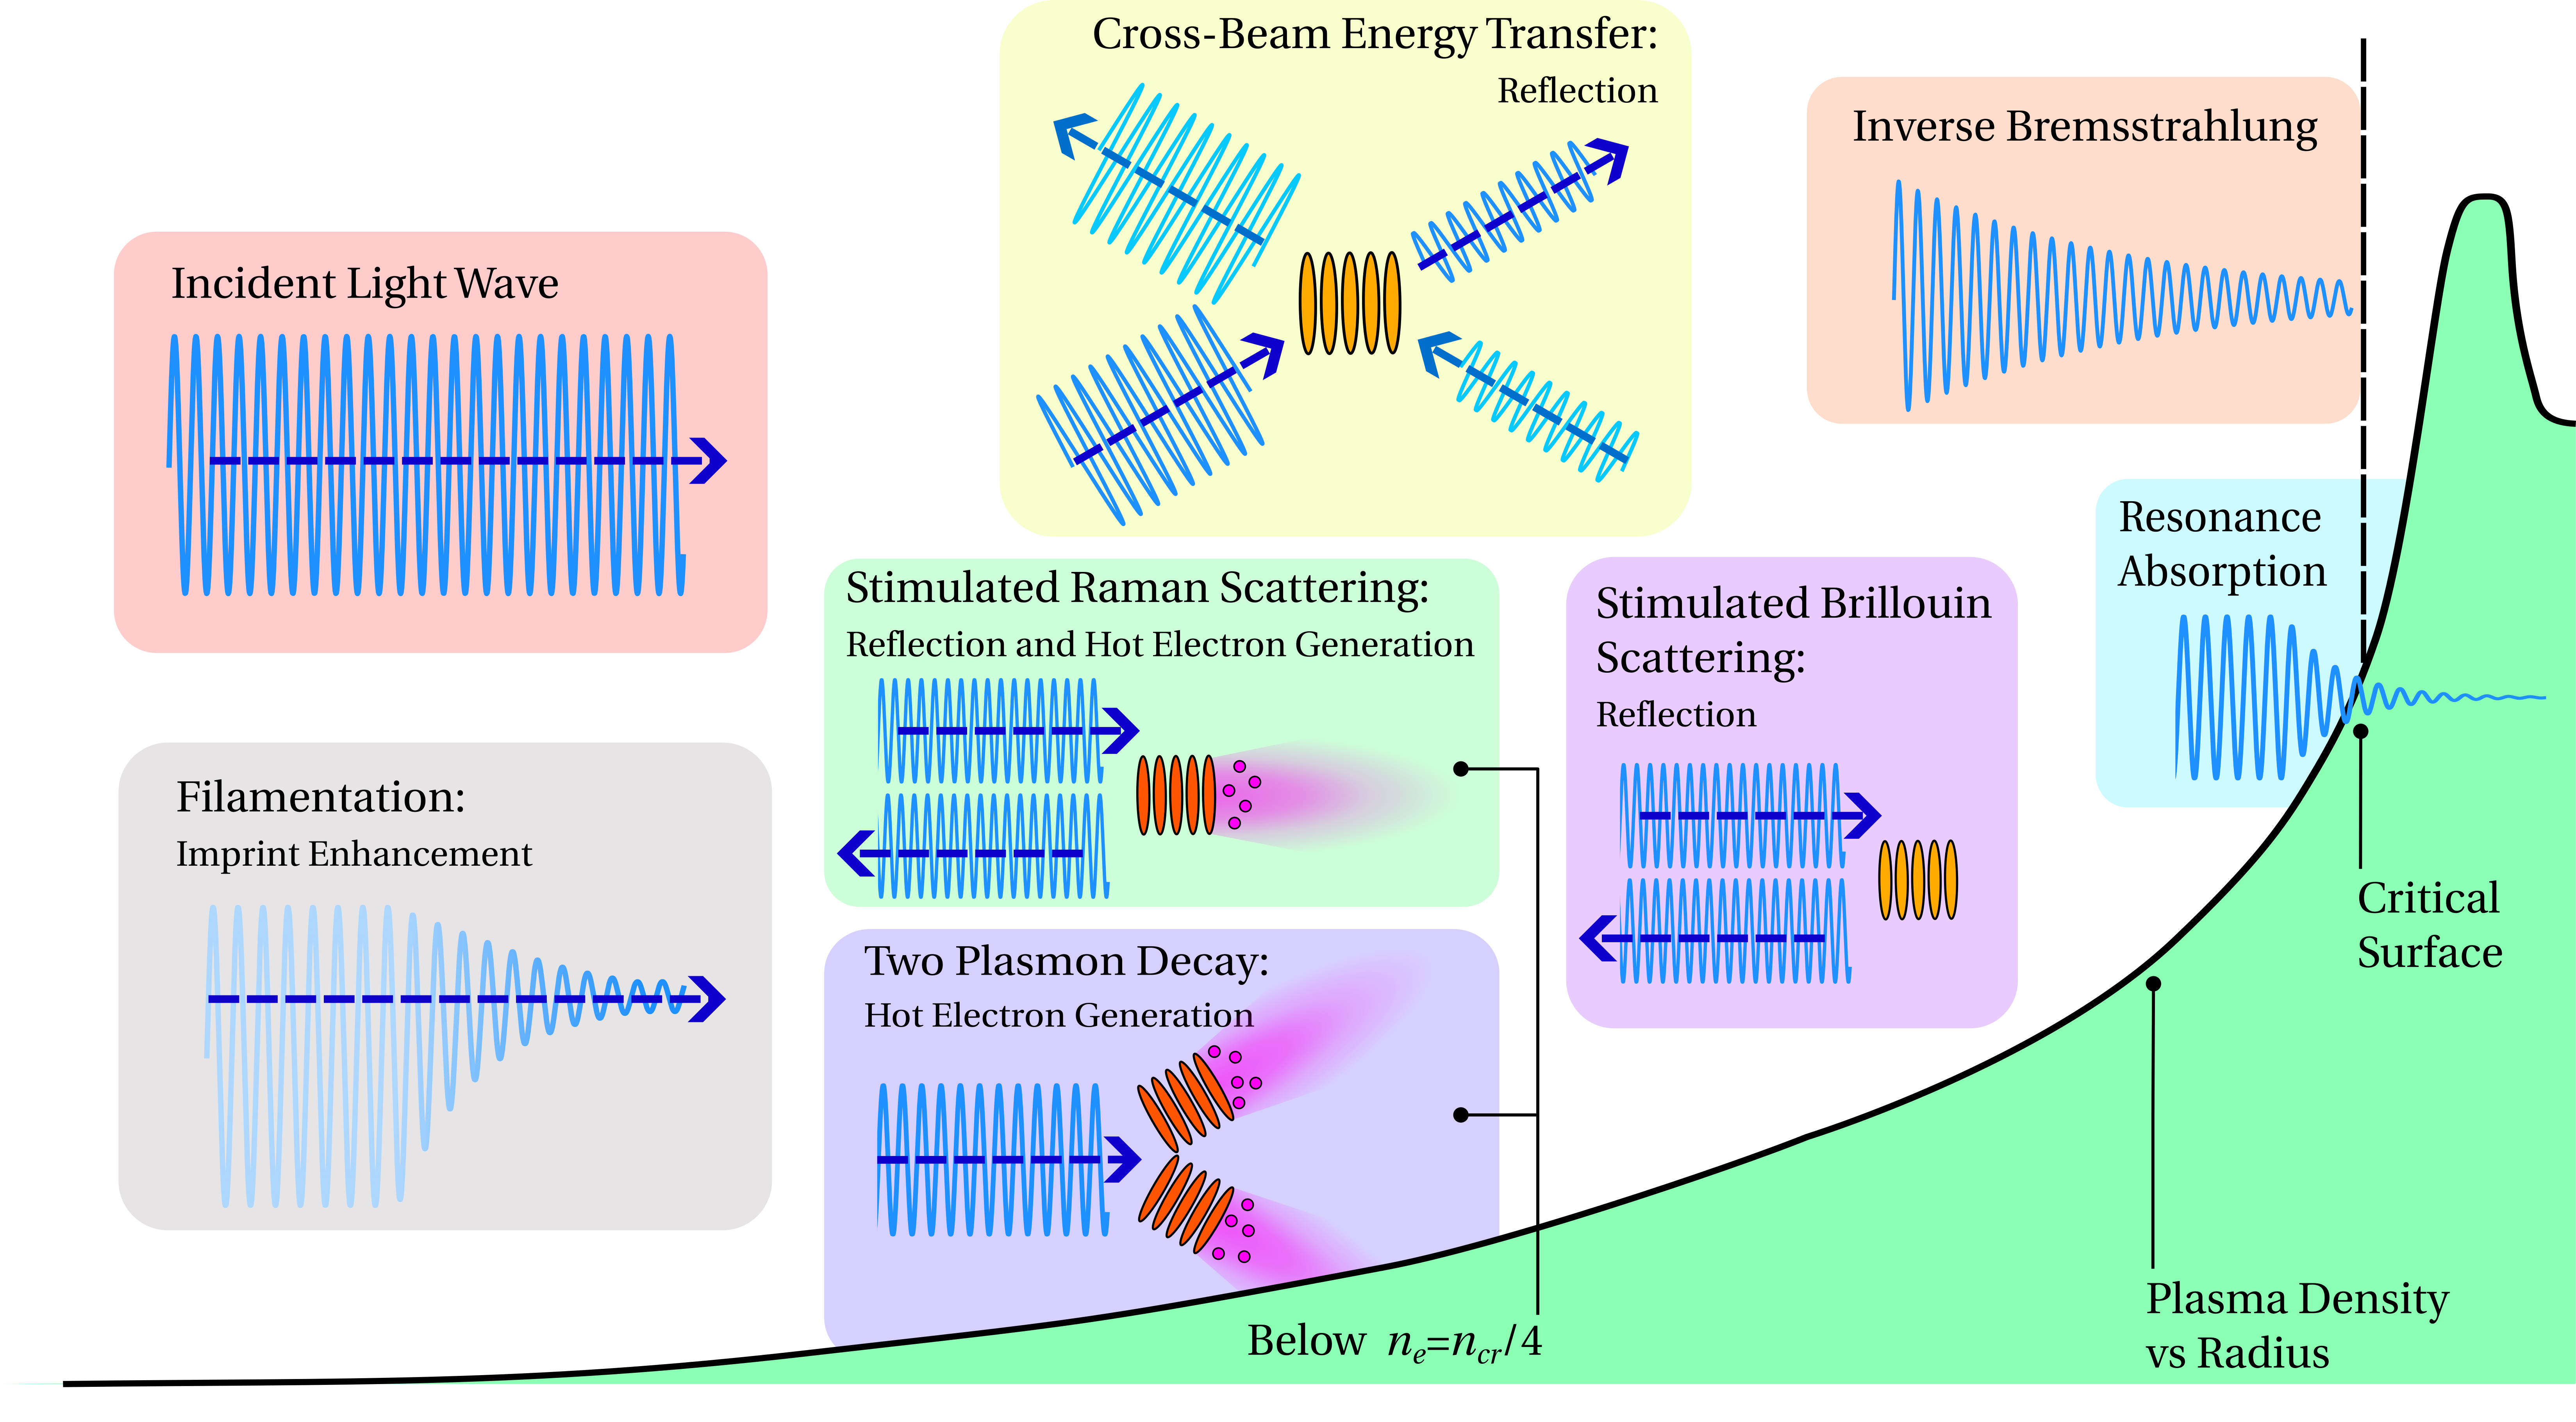
\includegraphics[width=\linewidth]{Introduction/Images/LPI diagram.png}
    \centering
    \caption{Important \ac{LPIs} for direct-drive \ac{ICF}.
    Energy is absorbed by \ac{Inv-Brem} close to critical, and resonance absorption at the critical surface.
    Hot electrons pre-heat the fuel reducing compressibility and are generated from an \ac{EPW} from \ac{TPD} or \ac{SRS}.
    Energy is reflected by \ac{CBET}, \ac{SRS} and \ac{SBS}.
    The filamentation instability can cause light to self-focus and thus enhance asymmetry of the deposition.
    }%
    \label{fig:intro_dd_lpis}
\end{figure}

\ac{LPIs} also act to significantly degrade direct-drive \ac{ICF} implosions.
A schematic diagram of \ac{LPIs} relevant to direct-drive is shown in Fig.~\ref{fig:intro_dd_lpis}.
Energy is absorbed either via \ac{Inv-Brem}, which is the absorption of laser energy by an electron while it undergoes a collision with an ion, or by resonance absorption, which is the excitation of a resonant \ac{EPW} at the critical surface.
\ac{Inv-Brem} is the dominant absorption mechanism for \textsc{Omega} experiments, because frequency-tripled\footnote{The \textsc{Omega} laser-beam are initially generated at a vacuum wavelength, $\lambda_0 = 1064\ \text{nm}$, by a Nd:YAG crystal and then passed through a non-linear optic, which converts the wavelength to $\lambda_0^{3\omega}=351\ \text{nm}$~\cite{boehly_upgrade_1995}.} light is employed for the lasers 
Similarly to indirect-drive, \ac{SBS} and \ac{SRS} act to reflect laser light away from the capsule.
However, unlike for indirect-drive, where \ac{CBET} is used to tune the symmetry of the implosion, in direct-drive configurations \ac{CBET} acts to reflect significant amounts of energy.
For direct-drive, the dominant \ac{CBET} interaction occurs as light from the edge of beams reflects outward and gains energy from inward travelling beams.
This mechanism is responsible for a $\sim20\%$ reduction in energy for typical \textsc{Omega} implosions over the whole implosion, and can instantaneously reduce power deposition by up to $\sim50\%$~\cite{colaitis_inverse_2021}.
Additionally, \ac{LPIs} which excite an \ac{EPW}, specifically \ac{TPD} and \ac{SRS}, can trap and accelerate a population of electrons to high energies ($\gtrsim50\ \text{keV}$), which travel through the ablator material and preheat the fuel, reducing compressibility and thus performance.
Finally, filamentation of the beam can occur, where the field self-focusses through low-density channels in the plasma, which increases laser non-uniformities~\cite{afshar-rad_evidence_1992}.

In central hotpot \ac{ICF} implosion, fusion reactions are made possible by a sufficiently hot and dense plasma hotspot, which is confined by the inertia of the target.
The energy required to assemble this hot and dense configuration occurs through a series of energy transfers.
\begin{itemize}
    \item Laser energy is converted to internal energy by absorption in the coronal plasma.
    \item This energy is coupled to kinetic energy in the shell by thermal conduction in the conduction zone.
    \item Kinetic energy of the shell stagnates on the axis, resulting in internal energy of the hotspot.
    \item This internal energy allows fuel reactants to overcome the Coulomb barrier and fuse, releasing binding energy as product kinetic energy.
\end{itemize}
The overall performance of implosions scales with the internal energy of the hotspot and can be improved, either by increasing the available driver energy, or by increasing the efficiency of these energy conversions.
The \textsc{Omega} laser facility has insufficient energy to achieve ignition conditions, thus inferring the performance of equivalent implosions on a larger laser direct-drive facility relies on techniques known as hydrodynamic scaling.
A combination of analytical methods and simulations are typically used to extrapolate the performance of \textsc{Omega} implosions to \ac{NIF} energies, $E_{\text{d}}\sim2\ \text{MJ}$, in order to compare performance of indirect- and direct-drive experiments~\cite{zhou_hydrodynamic_2007}.

Better hydrodynamic stability of the implosion improves the integrity of the imploding shell.
In analogy to a stiff piston compressing a gas, a denser and more uniform shell efficiently converts kinetic energy to internal energy of the hotspot gas, whereas a shell with short wavelength perturbations is effectively less dense and more compressible, decreasing conversion efficiency~\cite{betti_deceleration_2002}.
Over the past decade, implosion performance improved markedly by using statistical modelling techniques~\cite{lees_experimentally_2021}, to identify and reduce sources of yield degradation~\cite{lees_understanding_2023}.
Primarily by focussing on eliminating these short wavelength instabilities using the statistical model, fusion yield was tripled in a short period of time from $5\times10^{13}$ in 2016, to $1.5\times10^{14}$ in 2018~\cite{gopalaswamy_tripled_2019}\footnote{Improved instability robustness was achieved in these implosions, mostly by limiting the convergence ratio of the implosions.}.
The details of the statistical model used are discussed in Sec.~\ref{sec:Res1_OMEGA_stat_modelling}.

More recently, focus has also turned to increasing the efficiency of the energy conversion through other means.
Specifically, a significant fraction of laser energy remains unabsorbed, mostly due to \ac{CBET} can reduce power deposition instantaneously by $\sim50\%$.
\ac{CBET} has been reduced in recent campaigns via two means.
Firstly, `DT-liners' are an experimental configuration which have increased the outer diameter of the target, reducing the beam overlap and thus \ac{CBET}, which leads to high implosion velocities~\cite{williams_high_2021}.
This campaign recently reported for the first time that more fusion energy was produced, than was coupled to the hotspot.~\cite{williams_demonstration_2024}.
Secondly, a small amount ($\sim5\%$ by atomic number density) of silicon is now routinely added to the outer CH ablator.
This enhances the \ac{Inv-Brem} absorption of light, reducing the quantity of light that refracts away from the target, to act as a seed for \ac{CBET}.
Additionally, it reduces growth rates of many \ac{LPIs}, limiting the hot electron production.
A campaign which optimised the addition of silicon dopant recently demonstrated a hydrodynamically equivalent burning plasma on \textsc{Omega}, which is an important milestone on the path to hydrodynamically scaled ignition of a direct-drive implosion~\cite{gopalaswamy_demonstration_2024}.

%###############################################################################################################################
%###############################################################################################################################
%###############################################################################################################################
\section{Objective of the work}%
\label{sec:intro_objective}

Important physical processes in \ac{ICF} implosions occur on short time and length-scales, and have high temperatures and densities.
Inference of plasma conditions from escaping particles or radiation is thus typically used to understand the implosion dynamics.
However, these methods are limited to measuring emissive volumes at certain times throughout the experiments.
Simulations are an important tool, which are used to study \ac{ICF} experiments at greater spatial and temporal resolution than is allowed for by many diagnostic tools.
They can also be used to, for example, extrapolate the performance of experiments to larger facilities, or to help design new experiments~\cite{kritcher_design_2022}.
The applicability of simulations does of course depend upon the validity of the models used.
Hydrodynamics codes are the workhorse tool, used to simulate entire \ac{ICF} implosions.
The models employed in these codes must therefore be capable of accurately including relevant physical effects on long ($\sim\text{ns}$) timescales, which precludes many high fidelity, although expensive tools.

The aim of the work conducted in this thesis was to improve the modelling of the laser-plasma interactions in the 3-D \ac{MHD} code \textsc{Chimera}, particularly to more accurately simulate direct-drive \ac{ICF} experiments.
Prior to the work conducted in this thesis, a simple ray-tracing algorithm existed in \textsc{Chimera} to model the laser-plasma interaction, although it did not accurately account for refraction of the light.
Therefore, a simplified 1-D ray-trace was typically used for direct-drive calculations, where rays travelled radially inward and did not refract away from the target.
It was therefore deemed necessary to include a 3-D ray-trace, which accurately modelled the trajectory of laser light through the plasma and accounted for refractive coupling losses.

The discussion of indirect-drive in Sec.~\ref{sec:intro_indirect} and direct-drive in Sec.~\ref{sec:intro_direct} hopefully illustrated that \ac{LPIs} are a significant concern on current \ac{ICF} experiments.
Particularly \ac{CBET} in direct-drive is highly energetically significant, reducing the efficiency of laser absorption by $\sim20\%$ over the whole experiment.
Additionally, \ac{CBET} significantly alters deposition asymmetries~\cite{colaitis_inverse_2021}, and therefore it is crucial to accurately model the interaction, in order to understand the degradation of performance from multi-dimensional effects.
Despite this, few multidimensional \ac{CBET} models exist, which are suitable for direct-drive calculations, and only a single code, \textsc{Ifriit}, had been integrated to run inline with a 3-D hydrodynamics code~\cite{colaitis_inverse_2021}.
The second aim of the work was therefore to develop a \ac{CBET} model for the ray-trace which could be employed in direct-drive simulations and run inline with the hydrodynamics.

The remainder of this manuscript is organised as followed:
\begin{itemize}
    \item Chapter 2 introduces background theoretical material, relevant to the interaction of lasers with plasma in the regime of \ac{ICF}, with a particular focus on the techniques used in the computational models for work this thesis.
    Equations of the \ac{Rad-Hydro} framework are presented, alongside a discussion of their implementation in the \textsc{Chimera} code.
    A summary of the theory of the interaction of laser light with plasma is then presented, specifically the ray-tracing equations are introduced and their valifity discussed.
    Parametric instabilities, also known as \ac{LPIs} are finally discussed, with a particular emphasis on \ac{CBET}.
    
    \item Chapter 3 presents the 3-D laser ray-trace and \ac{CBET} module, \textsc{Solas}, which was developed for the \textsc{Chimera} code.
    
    
    \item Chapter 4
    
    \item Chapter 5
    
    \item Chapter 6
    
\end{itemize}
